\chapter{Results and Discussions}\label{ch:results}
This chapter is organized as follows: Section \ref{sec:result_data} will discuss the main data used in this study, including an illustration of how to access it and the features it provides; Section \ref{sec:ch4_desc_stat} will discuss the results of the descriptive statistics; Section \ref{sec:ch4_morphological_analysis} will discuss the results on the morphological analyses; Section \ref{sec:ch4_structural_analysis} will discuss the results on the structural analyses; Section \ref{sec:ch4_topic_modeling_result} will discuss the results of the topic modeling; and Section \ref{sec:ch4_relating_islamic_texts} will discuss the results of relating the Qur'\=an to other Islamic texts and analyses. Finally, Section \ref{sec:ch4_limitations} will discuss the limitations of the models used in this study.
\section{Theoretical Results}
The different analyses provided in this chapter were based on theoretical results of this paper, all of which are original contribution and are provided in the appendices. It will be discussed separately in the appendices to avoid cluttering this chapter with heavy mathematics that many Islamic scholars may not be familiar with. These results are provided in the appendices for reviewers and readers to see the details of the math behind the analyses.
\section{Qur'\=an Data}\label{sec:result_data}
The main data used in this study is the digitized Qur'\=an data available through QuranTree.jl library by \citeA{asaad2021qurantree}. QuranTree.jl has both the Tanzil data\footnote{\url{https://tanzil.net/}} and the Qur'anic Arabic Corpus\footnote{\url{https://corpus.quran.com/}}, where the latter contains the morphological data of the Qur'\=an. These digital data will help in doing programmatic analyses of the Qur'\=an using Julia programming language. To see how to access this in QuranTree.jl in Julia, Figure \ref{fig:result_crps_tbl} shows the code for accessing the morphological data of the first \arb[trans]{'ayaT} \arb{'ayaT} of \arb[trans]{sUraTu 'l-fAti.haT} \arb{sUraTu 'l-fAti.haT}. Note that, the setup on how to install the said QuranTree.jl and other libraries and the Julia programming language is given in Appendix \ref{appendix:installation_libraries}.

Referring to Figure \ref{fig:result_crps_tbl}, the first line of the code, which has the code \texttt{using QuranTree}, loads the QuranTree library. The second line, which has the code \texttt{crps, tnzl = load(QuranData())}, loads both the morphological data and the Tanzil data of the Qur'\=an. The third line of the code converts these data into a tabular form. Finally, the fourth line of the code queries the first \arb[trans]{sUraT} \arb{sUraT} and the first \arb[trans]{'ayaT} \arb{'ayaT} of the morphological data of the Qur'\=an, the results of which are shown in succeeding lines with the heading indicating \texttt{Chapter 1} and \texttt{Verse 1}. Both the number 1 for Chapter 1 is indicated by \texttt{[1]} and \texttt{[1]}, respectively, in the code \verb|crps_tbl[1][1]| in Figure \ref{fig:result_crps_tbl}.

\begin{figure}[!t]
    \centering
    \includegraphics[width=\textwidth]{img/crps_tbl.png}
    \caption{\arb[trans]{sUraTu 'l-fAti.haT} \arb{sUraTu 'l-fAti.haT} morphological data}
    \label{fig:result_crps_tbl}
\end{figure}

The output of the code in Figure 1 as indicated by the lines starting with \texttt{\#} shows the morphological data of the \textit{basmallah} \arb[fullvoc]{bismi 'l-l_ahi 'l-ra.hm_ani 'l-ra.hImi}. In this data, there are five columns after the Row column. The \texttt{word} column indicates the word of the queried data, in this case the first \arb[trans]{'ayaT} \arb{'ayaT} of the first \arb[trans]{sUraT} \arb{sUraT}. According to this column, there are four words in the \textit{basmallah}. The second column, \texttt{part}, indicates the parts of the word. In this case, the first word, has two parts. These two parts is indicated by its \texttt{form} in the third column, which are \texttt{bi} a Roman encoding based on Buckwalter mapping which is decoded in Arabic as \arb{bi}, and the second part of the first word has the form in Roman encoding through Buckwalter as \texttt{somi} or decoded in Arabic as \arb[fullvoc]{smi}. The fourth column indicates the part-of-speech of the parts of the words. For the first word, \arb[fullvoc]{bismi}, its two parts are composed of Preposition \arb{bi} and a Noun \arb[fullvoc]{smi}, both of which are further described in the \texttt{features} column, which is the morphological features column. In this last column, it further tells the reader that the Preposition \arb{bi} is a prefix. In addition, the second part \arb[fullvoc]{smi} is the stem of the word \arb[fullvoc]{bismi}, with lemma indicated by \texttt{\{som} which is decoded as \arb{"ism}, and a root of \arb{smw}. There are still other features detailed in the morphological column for the second word \arb[fullvoc]{smi}, and this can be described further using QuranTree.jl's \texttt{@desc} macro. The result of which is given in Figure \ref{fig:result_at_desc_basmallah}, which also show the other features such as the gender of the noun, in this case it is Masculine and is in Genitive case.

\begin{figure}[!t]
    \centering
    \includegraphics[width=\textwidth]{img/at_desc_basmallah.png}
    \caption{Morphological feature of the second part of the word \arb[fullvoc]{bismi}}
    \label{fig:result_at_desc_basmallah}
\end{figure}

The Quranic Arabic Corpus data which contain the morphological features discussed above, has the Qur'\=an texts represented as Buckwalter encoding, which is a character by character mapping of the Arabic orthographies of the Qur'\=an into a Roman letter. This encoding if decoded to Arabic matches exactly the Qur'\=an \arb[trans]{mu.s.haf} \arb{mu.s.haf}. In fact, the Tanzil data which is also available in QuranTree.jl, exactly matches this data. The difference between the two is that the Tanzil data only contains the Arabic texts of the Qur'\=an broken down up until the \arb[trans]{'ayaT} \arb{'ayaT} only. Figure \ref{fig:result_tnzl_tbl} shows the Tanzil data queried through the QuranTree.jl for \arb[trans]{sUraTu 'l-fAti.haT} \arb{sUraTu 'l-fAti.haT}. The only difference between the two data in terms of presentation of the \arb[trans]{sUraT} \arb{sUraT} is that, the Quranic Arabic Corpus (in Figure \ref{fig:result_crps_tbl}) skips the \textit{basmallah} for all \arb[trans]{sUwar} \arb{sUwar} except for the first, \arb[trans]{sUraTu 'l-fAti.haT} \arb{sUraTu 'l-fAti.haT}, while the Tanzil data has it in every \arb[trans]{sUwar} \arb{sUwar}.

\begin{figure}[!t]
    \centering
    \includegraphics[width=\textwidth]{img/tnzl_tbl.png}
    \caption{\arb[trans]{sUraTu 'l-fAti.haT} \arb{sUraTu 'l-fAti.haT} Tanzil data}
    \label{fig:result_tnzl_tbl}
\end{figure}

The rich data available in QuranTree.jl opens up many possibilities for researchers to do programmatic analyses of the Qur'\=an. Especially on the use of Statistical modeling to understand its structure and patterns. This paper will demonstrate some of these possibilities. The data can be used to do morphological analyses, structural analyses, and even topic modeling. The data can also be used to do other analyses such as sentiment analysis, and other text analytics. 

\section{Descriptive Statistics}\label{sec:ch4_desc_stat}
The first statistical analysis is to describe the distribution of the data, through Descriptive Statistics. This statistical method is mainly used to summarize the data by looking at the central tendency, dispersion, and shape of the distribution of the data. The central tendency is a measure of the center of the data, which can be represented by the mean, median, and mode. The dispersion is a measure of how spread out the data is, which can be represented by the range, variance, and standard deviation.

The data in this case are the orthographies, parts of words, words, \arb[trans]{ayAt} \arb{ayAt}, and \textit{s\=urah} \arb{sUraT} of the Qur'\=an. The Qur'\=an is a collection of 114 \textit{s\=urah} \arb{sUraT} and 6,348 \arb[trans]{ayAt} \arb{ayAt}. Each \textit{s\=urah} \arb{sUraT} is made up of a number of \arb[trans]{ayAt} \arb{ayAt}, and each \arb[trans]{ayAt} \arb{ayAt} is made up of a number of words, which in turn is made of parts, and finally parts are made up of Arabic letters. These data as discussed in the previous section are available through the Quranic Arabic Corpus and the Tanzil data in the QuranTree.jl library.

As discussed in the Introduction of this thesis, the Qur'\=an has unique organizational structure unlike other scriptures. This has attracted both Muslims and non-Muslims to endeavor on understanding its structure. Most of the scholars have done this manually, going through each \arb[trans]{ayAt} \arb{ayAt} and \arb[trans]{sUraT} \arb{sUraT} of the Qur'\=an one at a time to find patterns that will at least convey why it is arranged as it is. However, this manual process is very tedious and time consuming, and hence other opportunities to understanding its structure has not yet been explored. Among those is undersanding the statistics of the counts of the words, \arb[trans]{AyAt} \arb{AyAt}, and \arb[trans]{suwar} \arb{suwar}. 

\begin{figure}[!t]
    \centering
    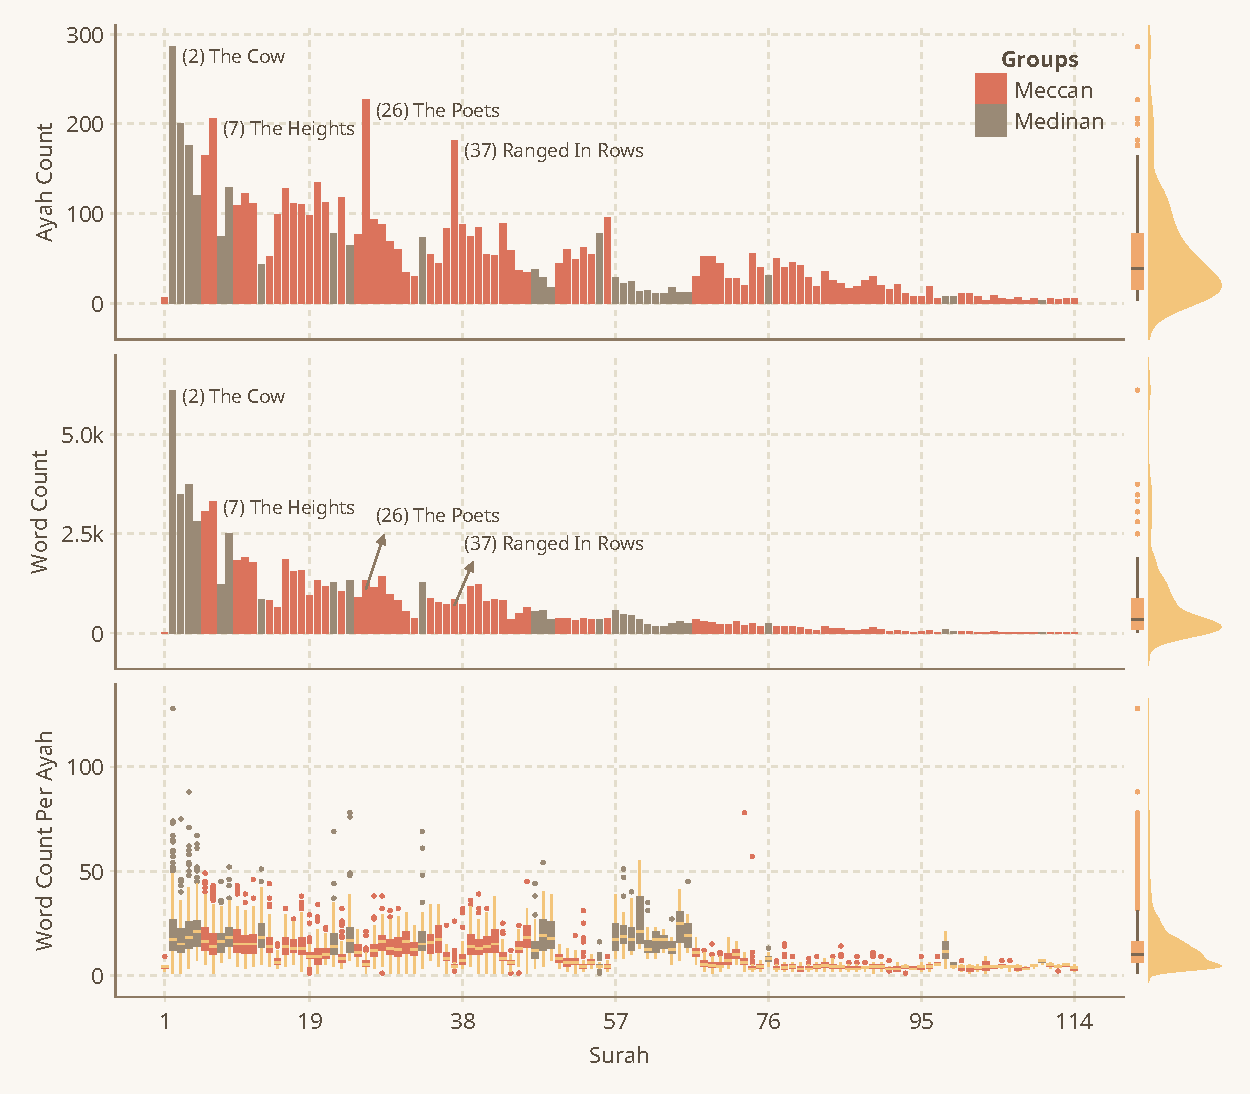
\includegraphics[width=\textwidth]{img/plot1.pdf}
    \caption{Distribution of Meccan and Medinan \arb[trans]{sUwar} \arb{sUwar}}
    \label{fig:result_ayah_word_count}
\end{figure}

Figure \ref{fig:result_ayah_word_count} shows the bar chart of the \arb[trans]{AyAt} \arb{AyAt} counts and word counts, and also the distribution of the word counts and character counts both per \arb[trans]{ayAt} \arb{ayAt}. In this figure, the geographical locations (Meccan or Medinan) of the \arb[trans]{sUraT} \arb{sUraT} based on the \arb[trans]{'asbAb 'alnuzUl} \arb{'asbAb 'alnuzUl} or the 'occasions/circumstances of revelation' are also indicated.

The first obvious pattern, which is known to Muslims, is the monotonically decreasing number of the \arb[trans]{ayAt} \arb{ayAt} after the first \arb[trans]{sUraT} \arb{sUraT}. This is true for both the bar charts of the \arb[trans]{ayAt} \arb{ayAt} count and the word count. An interesting pattern also is that, two \arb[trans]{suwar} \arb{suwar} has significant number of \arb[trans]{AyAt} \arb{AyAt} but with each \arb[trans]{ayAt} \arb{ayAt} having small number of words. These two \arb[trans]{suwar} \arb{suwar} are the \arb[trans]{sUraT} \arb{sUraT} 26th (\arb[trans]{sUraTu 'l-^su`arA'} \arb{sUraTu 'l-^su`arA'} or "the Poet") and 37th (\arb[trans]{sUraTu 'l-.sAffAt} \arb{sUraTu 'l-.sAffAt} or "the Ranged in Rows"), respectively. This can be confirmed even in the Medina Mushaf, where the first page for \arb[trans]{sUraTu 'l-^su`arA'} \arb{sUraTu 'l-^su`arA'} already contains 19 \arb[trans]{AyAt} \arb{AyAt}, and the \arb[trans]{sUraTu 'l-.sAffAt} \arb{sUraTu 'l-.sAffAt} contains 24 \arb[trans]{AyAt} \arb{AyAt} in its first page. This indicates that the said \arb[trans]{suwar} \arb{suwar} contain small number of words per \arb[trans]{ayAt} \arb{ayAt} shown in Figure \ref{fig:result_ayah_word_count}.

Moving on, the distribution of the words per \arb[trans]{ayAt} \arb{ayAt} and the characters per \arb[trans]{ayAt} \arb{ayAt} are shown in the third and fourth rows or plots of Figure \ref{fig:result_ayah_word_count}. It is indeed expected that these distributions are more or less identical, since it is expected that more words means more characters. The reason why the distribution of characters per \arb[trans]{ayAt} \arb{ayAt} is shown is to make it comparable to the work of \citeA{sinai2020oqs}, which will be compared later in Section. 

To interpret these distributions of word count per \arb[trans]{ayAt} \arb{ayAt} and the character count per \arb[trans]{ayAt} \arb{ayAt}, the $x$-axis is still the 114 \arb[trans]{suwar} \arb{suwar} of the Qur'\=an, while the $y$-axis is either the count of words (third row plot) per \arb[trans]{ayAt} \arb{ayAt} or the count of characters (fourth row plot) per \arb[trans]{ayAt} \arb{ayAt} in Figure \ref{fig:result_ayah_word_count}. Thus, each boxplot shown in these plots describes the distributions of the count of either the words or characters per \arb[trans]{ayAt} \arb{ayAt}. From these distributions, an interesting groups of distributions at around 57th \arb[trans]{sUraT} \arb{sUraT} to 66th \arb[trans]{sUraT} \arb{sUraT} are observed. These distributions while might be reasoned as easily seen because of its Medinan \arb[trans]{'asbAb 'alnuzUl} \arb{'asbAb 'alnuzUl} color, the mean of these are obviously higher than its surrounding \arb[trans]{sUraT} \arb{sUraT} as seen in the figure. In fact, these \arb[trans]{suwar} \arb{suwar} have lower number of \arb[trans]{ayAt} \arb{ayAt} compared to its surrounding \arb[trans]{suwar} \arb{suwar} (\textit{see} first plot and second plot of Figure \ref{fig:result_ayah_word_count}). Although, the number of words are more or less the same.

Further, it can be observed that the distributions of the Medinan \arb[trans]{suwar} \arb{suwar} tend to have higher mean as opposed to those in Meccan \arb[trans]{suwar} \arb{suwar}, which is indeed the case as seen in later discussions. In fact, as a prelude to this, if the order of the arb[trans]{suwar} \arb{suwar} is based on the \arb[trans]{'asbAb 'alnuzUl} \arb{'asbAb 'alnuzUl}, the observation that Medinan surah has higher number of word or character per \arb[trans]{ayAt} \arb{ayAt} can be seen in Figure \ref{fig:result_ayah_word_count_rev_order}. In this figure, the Medinan \arb[trans]{suwar} \arb{suwar} seen in the latter part of the \arb[trans]{'asbAb 'alnuzUl} \arb{'asbAb 'alnuzUl} clearly have higher mean counts and tend to have variable number of word or character counts per \arb[trans]{ayAt} \arb{ayAt}. This is again true especially when looking at the overall distributions of these categories across \arb[trans]{suwar} \arb{suwar} as in Figure \ref{fig:result_meccan_medinan_dist}.

\begin{figure}[!t]
    \centering
    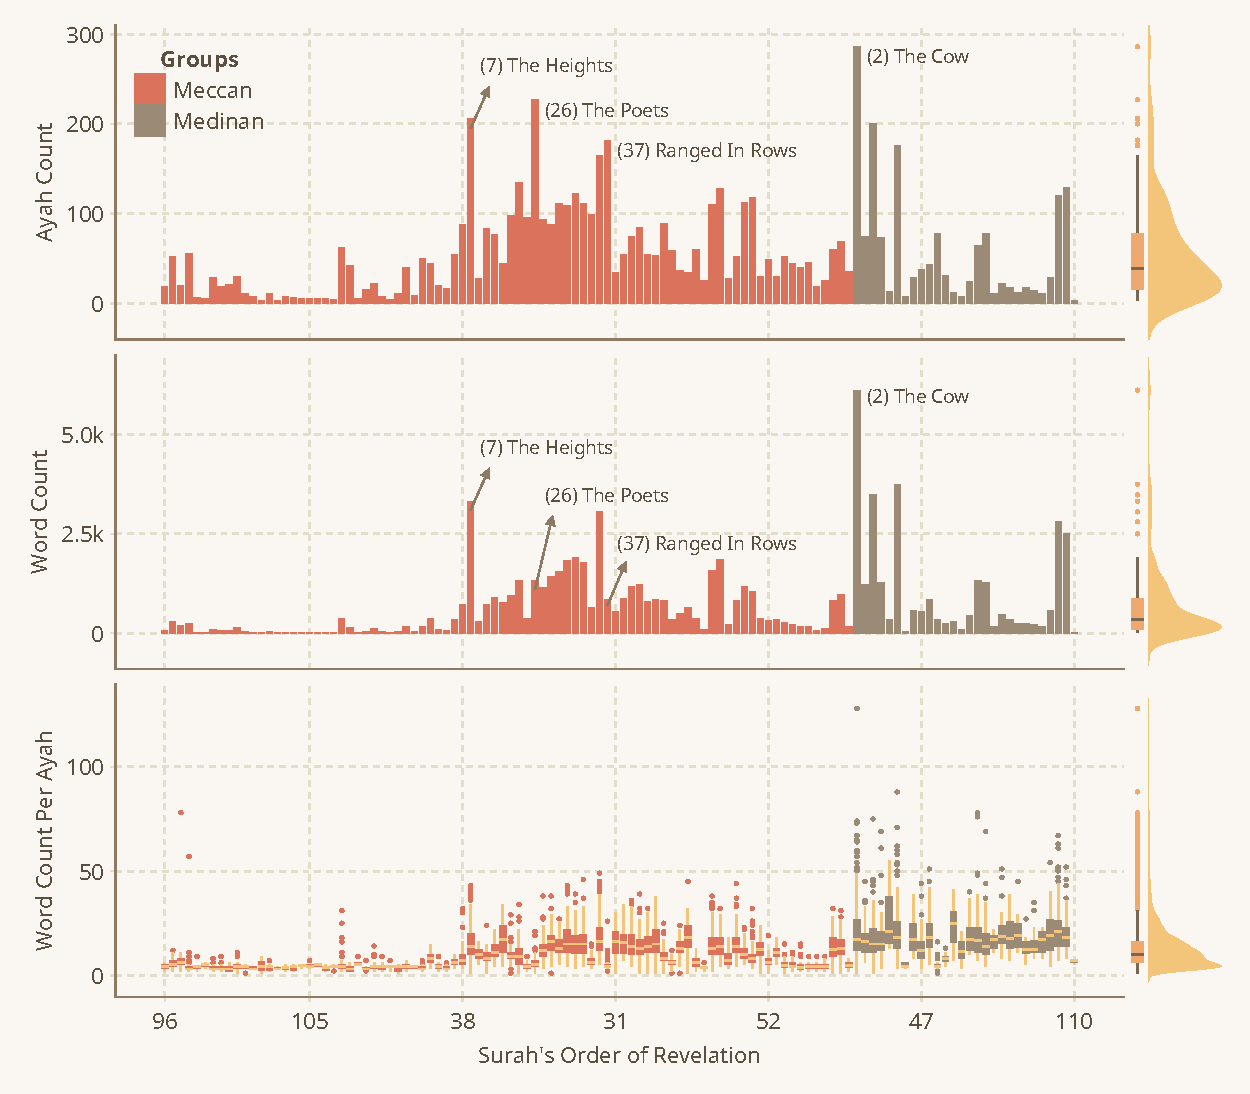
\includegraphics[width=\textwidth]{img/plot2.pdf}
    \caption{Statistics of the words and \arb[trans]{ayAt} \arb{ayAt} (verses) of the Qur'\=an according to revelation order}
    \label{fig:result_ayah_word_count_rev_order}
\end{figure}

\begin{figure}[!t]
    \centering
    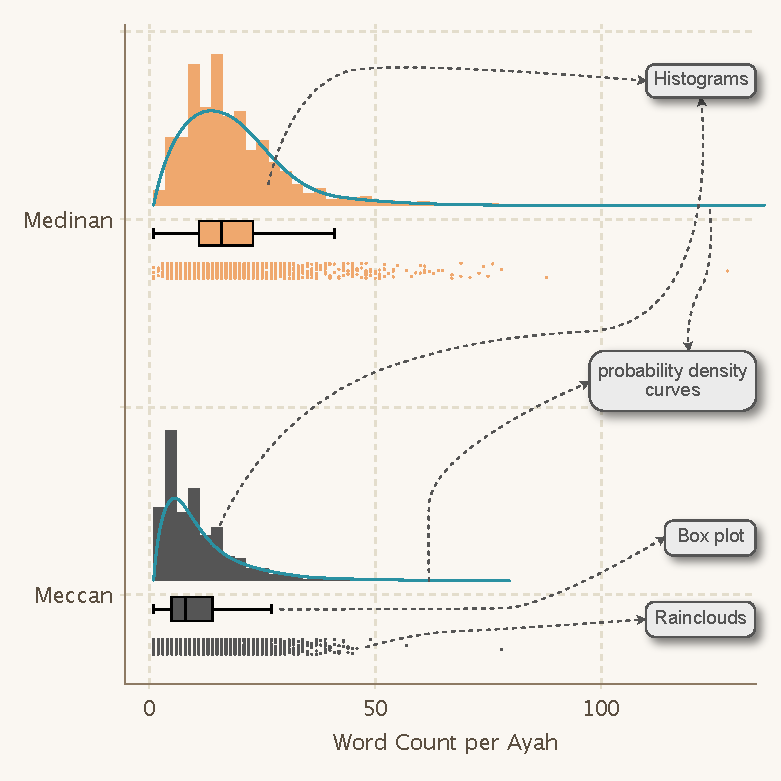
\includegraphics[width=\textwidth]{img/plot3.pdf}
    \caption{Distribution of Meccan and Medinan \arb[trans]{sUwar} \arb{sUwar}}
    \label{fig:result_meccan_medinan_dist}
\end{figure}

\begin{table}
    \caption{Descriptive statistics of the \arb[trans]{ayAt} \arb{ayAt} counts and the counts of its words}
    \label{tbl:desc_stats}
    \begin{tabularx}{\textwidth}[!h]{XXXX}
        \toprule
        Count Data&Mean&Median&Std. Deviation\\
        \midrule
        Ayahs&54.70&39&53.21\\
        Words&679.20&344&931.18\\
        Words per Ayah&10.27&8.23&6.35\\
        \bottomrule
    \end{tabularx}
\end{table}
\subsection{Comparison to Sinai's Inner-Chronology}
The work of \citeA{sinai2020oqs} investigated the same statistical distributions as in the previous section, but has focused from a non-traditionalist view by not basing on the \arb[trans]{'asbAb 'alnuzUl} \arb{'asbAb 'alnuzUl}, and instead mainly on the Qur'\=an's text itself using a transliteration data from Prof. Hans Zirker. The said data is not exactly the same as the one used in here, nor it is publicly verified as the one (Quranic Arabic Corpus and the Tanzil data) used in this study. Nonetheless, if indeed the said transliteration is exactly the same as the one used here once decoded to its Arabic form, the result should more or less be the same. However, while the preprocessing done by \citeA{sinai2020oqs} was not done in the analyses of the previous section, the result of the distributions should not deviate much. In the said study of \citeA{sinai2020oqs}, the findings suggest that there is inner-chronology of the Qur'\=an. This was concluded by the said author by looking at the mean verse length, which is more or less similar to the median verse length indicator used in boxplots of the third and fourth plots of Figures \ref{fig:result_ayah_word_count} and \ref{fig:result_ayah_word_count_rev_order}. Indeed, median is a better metric than mean in this case due to outlier counts seen in the boxplots in Figures \ref{fig:result_ayah_word_count} and \ref{fig:result_ayah_word_count_rev_order}. It is surprising though that he considered those with significant variance or coefficient variations (meaning those \arb[trans]{suwar} \arb{suwar} with very varied number of characters per \arb[trans]{ayAt} \arb{ayAt}) as possible later insertion to the Qur'\=an upon his closer inspection. It may sound polemic to disregard his findings or to attack it, but to be fair to Muslim traditionalists that to believe in such claim requires solid evidence from extant manuscripts and not just from someone's own interpretation of the statistics or literary styles of the \arb[trans]{ayAt} \arb{ayAt}. Indeed, the findings of Prof. Sina's can be categorized as \textit{theories} as it does not have supporting manuscripts that shows one. It may also be difficult to prove so as all Qur'\=anic extant manuscripts are consistent with the current one, including the controversial Sana'a Palimpest, where also Prof. Sinai was fair to admit in his own book \cite{sinai2017} that the said texts have. 

Furthermore, while it is healthy for the advancement of any studies including Qur'\=anic studies to have opposing views. For the case of \citeA{sinai2020oqs}, the premise of not considering \arb[trans]{'asbAb 'alnuzUl} \arb{'asbAb 'alnuzUl} shows a different structure as discussed in the preceding section.
\section{Morphological Analysis}\label{sec:ch4_morphological_analysis}
The second statistical analysis is to analyze the morphological features of the Qur'\=an. There are several ways to do this, and the easiest one is to find a particular word and study its morphologies. This will be the goal of this section, and the important word to study is the name of God in the Qur'\=an and that is \arb[trans]{'l-l_ah} \arb{'l-l_ah}. The root of this word is the \arb[trans]{Alh} \arb[novoc]{Alh}, and thus the morphologies of this root word will be studied and compared againts the \arb[trans]{'asbAb 'alnuzUl} \arb{'asbAb 'alnuzUl} or the 'occasions/circumstances of revelation.' Table \ref{tbl:result_Alh_morphologies} contains the complete list of morphologies of \arb[trans]{Alh} \arb[novoc]{Alh}. The first column in the said table lists the said morphologies, the second column lists its location in \arb[trans]{sUraT} \arb{sUraT} and \arb[trans]{'ayaT} \arb{'ayaT}, the third column lists the total number of \arb[trans]{'ayaT} \arb{'ayaT} that has the said morphology in the Qur'\=an, and the fourth column lists the percentage of \arb[trans]{'ayaT} \arb{'ayaT} whose \arb[trans]{'asbAb 'alnuzUl} \arb{'asbAb 'alnuzUl} is Mecca. The codes on how to generate this table in Julia using QuranTree.jl, Yunir.jl, and DataFrames.jl libraries are shown in Figure \ref{fig:result_Alh_morphologies}.

\begin{table}[!t]
    \begin{tabularx}{\textwidth}[!h]{cXcc}
        \toprule\\[-0.3cm]
        Morph. & Surah \& Ayah & Count & Meccan \% \\[0.2cm]
        \midrule\\[-0.4cm]
        \arb[fullvoc]{'l-l_ahi} & 1:1, 2:8, 2:23, $\cdots$, 104:6, 110:1, 110:2 & $710$ & 47\% \\[0.2cm]
        \arb[fullvoc]{llahi} & 1:2, 2:22, 2:98, $\cdots$, 71:13, 72:18, 82:19 & $122$ & 55\%\\[0.2cm]
        \arb[fullvoc]{'l-l_ahu} & 2:7, 2:10, 2:15, $\cdots$, 98:8, 112:1, 112:2 & $624$ & 39\% \\[0.2cm]
        \arb[fullvoc]{'l-l_aha} & 2:9, 2:26, 2:55, $\cdots$, 72:12, 96:14, 98:5 & $351$ & 30\% \\[0.2cm]
        \arb[fullvoc]{'il---a---_aha} & 2:133, 3:6, 6:106, $\cdots$, 45:23, 47:19, 73:9 & $17$ & 76\% \\[0.2cm]
        \arb[fullvoc]{'il---a---_ahu} & 2:163, 16:22, 18:110, $\cdots$ , 21:108, 29:46, 41:6 & $8$ & 88\% \\[0.2cm]
        \arb[fullvoc]{'il---a---_ahiN} & 3:62, 28:38, 38:65 & $3$ & 67\%\\[0.2cm]
        \arb[fullvoc]{|"'AlihaTaN} & 6:74, 18:15, 21:21, $\cdots$, 36:23, 37:86, 43:45 & $9$ & 100\% \\[0.2cm]
        \arb[fullvoc]{|"'Alihata} & 7:127, 21:36, 21:68, 71:23 & $4$ & 100\% \\[0.2cm]
        \arb[fullvoc]{'il---a---_ahaN} & 7:138, 18:14, 26:29 & $3$ & 100\%\\[0.2cm]
        \arb[fullvoc]{|"'Alihati} & 11:53, 11:54, 19:46, 25:42, 37:36, 37:91, 38:6, 46:22 & $8$ & 100\% \\[0.2cm]
        \arb[fullvoc]{|"'Alihatu} & 11:101 & $1$ & 100\% \\[0.2cm]
        \arb[fullvoc]{'il---a---_ahuN} & 14:52, 21:29, 43:84, 52:43 & $4$ & 100\% \\[0.2cm]
        \arb[fullvoc]{|"'AlihaTuN} & 17:42, 21:22, 21:43 & $3$ & 100\% \\[0.2cm]
        \arb[fullvoc]{'il---a---_ahi} & 20:97, 40:37, 114:3 & $3$ & 100\% \\[0.2cm]
        \arb[fullvoc]{--|"'Alihati}& 21:59, 21:62 & $2$ & 100\%\\[0.2cm]
        \arb[fullvoc]{|"'il---a---_ahuN} & 27:60, 27:61, 27:62, 27:63, 27:64 & $5$ & 100\% \\[0.2cm]
        \arb[fullvoc]{|"'AlihaTa} & 38:5 & $1$ & 100\% \\[0.2cm]
        \arb[fullvoc]{'alihatu} & 43:58 & $1$ & 100\% \\[0.2cm]
        \bottomrule
    \end{tabularx}
    \caption{Morphologies of \arb[novoc]{Alh} in the Qur'\=an}
    \label{tbl:result_Alh_morphologies}
\end{table}

The codes in Figure \ref{fig:result_Alh_morphologies} defines a Julia function called \verb|get_morphologies| from lines 5 to 25. The body of this function contains logics for extracting the morphologies of a given root word. At a high level, the logics has the following flow: it reads the morphological features of the root word \arb[novoc]{Alh}, then it lists down the chapter and verses containing this root word, and then compute the total number of \arb[trans]{AyAt} \arb{AyAt} that contain the given morphology of the given root word. Finally, it returns the output in tabular form that is presented in Table \ref{tbl:result_Alh_morphologies}. The defined \verb|get_morphologies| function can then be used to generate similar tables from other root words without rewriting those codes in lines 5 to 25 of Figure \ref{fig:result_Alh_morphologies}. Indeed, this is the beauty of programming, it can automate the manual process. For example, to generate similar table for the morphology of \arb{r.hm}, the code is as simple as shown in Figure \ref{fig:result_rHm_morphologies}, which shows only the first five morphologies of \arb{r.hm}.

\begin{figure}[!t]
    \centering
    \includegraphics[width=\textwidth]{img/morphologies_Alh.png}
    \caption{Julia code for generating Table \ref{tbl:result_Alh_morphologies}}
    \label{fig:result_Alh_morphologies}
\end{figure}

\begin{figure}[!t]
    \centering
    \includegraphics[width=\textwidth]{img/morphologies_rHm.png}
    \caption{Julia code for generating morphologies of \arb[novoc]{r.hm}}
    \label{fig:result_rHm_morphologies}
\end{figure}

From the result it can be observed that those these morphologies are purely under Meccan: \arb[trans]{'alihatu}  \arb[fullvoc]{'alihatu} - a masculine plural noun in nominative case (\textit{see} Figure \ref{fig:result_mfeat_43_58} for the codes on how to get these details in QuranTree.jl); \arb[trans]{|"'AlihaTa} \arb[fullvoc]{|"'AlihaTa} - a masculine plural noun in accusative case; \arb[trans]{|"'il---a---_ahuN} \arb[fullvoc]{|"'il---a---_ahuN} - a masculine singular noun in indefinite state and nominative case; \arb[trans]{--|"'Alihati} \arb[fullvoc]{--|"'Alihati} - a masculine plural noun in genitive case; \arb[trans]{'il---a---_ahi} \arb[fullvoc]{'il---a---_ahi} - a masculine singular noun in genitive case; \arb[trans]{|"'AlihaTuN} \arb[fullvoc]{|"'AlihaTuN} - a masculine plural noun in indefinite state and nominative case; \arb[trans]{'il---a---_ahuN} \arb[fullvoc]{'il---a---_ahuN} - similar to \arb[trans]{|"'il---a---_ahuN} \arb[fullvoc]{|"'il---a---_ahuN} with slightly different morphology; \arb[trans]{|"'Alihatu} \arb[fullvoc]{|"'Alihatu} - a masculine plural noun in nominative case; \arb[trans]{|"'Alihati} \arb[fullvoc]{|"'Alihati} - a masculine plural noun in genitive case; \arb[trans]{'il---a---_ahaN} \arb[fullvoc]{'il---a---_ahaN} - a masculine singular noun in indefinite state and accusative case; \arb[trans]{|"'Alihata} \arb[fullvoc]{|"'Alihata} - a masculine plural noun in accusative state, \arb[trans]{|"'AlihaTaN} \arb[fullvoc]{|"'AlihaTaN} - a masculine plural noun in indefinite state and accusative case.

\begin{figure}[!t]
    \centering
    \includegraphics[width=\textwidth]{img/mfeat_43_58.png}
    \caption{Julia code for describing morphological features of \arb[trans]{'alihatu} \arb{'alihatu}}
    \label{fig:result_mfeat_43_58}
\end{figure}

The last column in Table \ref{tbl:result_Alh_morphologies} contains the percentages of the Meccan \arb[trans]{AyAt} \arb{AyAt}, therefore among the \arb[trans]{AyAt} \arb{AyAt} that contain the morphologies of \arb[trans]{'l-l_ahi} \arb[fullvoc]{'l-l_ahi} is that 47\% of those are Meccan. This column was generated by the code in Figure \ref{fig:result_meccan_ratio}.

\begin{figure}[!t]
    \centering
    \includegraphics[width=\textwidth]{img/meccan_ratio.png}
    \caption{Julia code for generating last column of Table \ref{tbl:result_meccan_ratio}}
    \label{fig:result_meccan_ratio}
\end{figure}

Sample \arb[trans]{AyAt} \arb{AyAt} are given for Q43:59, Q21:59, and Q2:23. The first \arb[trans]{'ayaT} \arb{'ayaT} contains the only morphology for \arb[trans]{'alihatu} \arb[fullvoc]{'alihatu} in the Qur'\=an, which is highlighted in red. The context of this \arb[trans]{'ayaT} \arb{'ayaT} is that it the \textit{gods} (\arb[trans]{'alihatu} \arb[fullvoc]{'alihatu}) referred here are the dieties worshipped by the disbelievers. The one they cited here as \textit{him} is given in the previous  \arb[trans]{'ayaT} \arb{'ayaT} as Jesus \txarb{\fontspec{Scheherazade New} ﵇}, the son of Mary \txarb{\fontspec{Scheherazade New} ﵍}. 

\begin{bottomtitledframe}{Q43:58}
    \begin{center}
        \begin{arab}[fullvoc]
            min ((sUraTu 'l-zuxrufi)): waqAlUA |"'a\arbcolor[red]{'a_alihatu}nA xayruN 'am huwa mA .darabUhu laka 'illA jadalA bal hum qawmun xA.simUn
        \end{arab}
        \begin{arab}[trans]
            min ((sUraTu 'l-zuxrufi)): waqAlUA |"'a\arbcolor[red]{'a_alihatu}nA xayruN 'am huwa mA .darabUhu laka 'illA jadalA bal hum qawmun xA.simUn
        \end{arab}
    \end{center}
    From Surah \textit{Ornaments of Gold}: saying, 'Are our \textcolor{red}{gods} better or him?' --- they cite him only to challenge you: they are a contentious people ---
\end{bottomtitledframe}

The next Meccan \arb[trans]{'ayaT} \arb{'ayaT} is Q21:59, which contain the morphology for \arb[trans]{--|"'Alihati} \arb[fullvoc]{--|"'Alihati}, which refers to \textit{gods} or \textit{deities} of the disbelievers. In this \arb[trans]{'ayaT} \arb{'ayaT} the question is coming from disbelievers during the time of Abraham \txarb{\fontspec{Scheherazade New} ﵇}, after he destroyed the idols worshipped by his father and the disbelievers. Indeed, the not so common morphologies for \arb[novoc]{alh} refer to false gods and dieties and not to the true God that the Qur'\=an refers to. 

\begin{bottomtitledframe}{Q21:59}
    \begin{center}
        \begin{arab}[fullvoc]
            min ((sUraTu 'l-'anbiyA'i)): waqAlUA man fa`ala ha_a_dA bi\arbcolor[red]{--|"'Alihati}n'A 'innahu lamina 'l-.za_alimIna
        \end{arab}
        \begin{arab}[trans]
            min ((sUraTu 'l-'anbiyA'i)): waqAlUA man fa`ala ha_a_dA bi\arbcolor[red]{--|"'Alihati}n'A 'innahu lamina 'l-.za_alimIna
        \end{arab}
    \end{center}
    From Surah \textit{The Prophets}: They said, 'Who has done this to our \textcolor{red}{gods}? How wicket he must be!
\end{bottomtitledframe}

Finally, the example for the use of \arb[novoc]{alh} morphology to refer to the true God in the Qur'\=an is given in Q2:23, for \arb[trans]{'l-lahi} \arb[fullvoc]{'l-lahi}. Here the context is the challenge of Allah or God to the disbelievers to produce a single \textit{s\=urah} \arb{sUraT} or chapter like that in the Qur'\=an. This is indeed a challenge that is still valid until today, and no one has ever produced a single \textit{s\=urah} \arb{sUraT} like the Qur'\=an. If there was one, it should have been published in a reputable journal addressing this challenge. The problem with producing this is that it should be with the same eloquence and beauty of the Qur'\=an. This is indeed a challenge that is still valid until today, and no one has ever produced a single \textit{s\=urah} \arb{sUraT} like the Qur'\=an. This is part of the \arb[trans]{'al-'i`jAzu 'l-qur`an} \arb{'al-'i`jAzu 'l-qur`an} or \textit{the inimitability of the Qur'\=an}, which is one of the main reasons why the Qur'\=an is considered to be a miracle by the Muslims.

\begin{bottomtitledframe}{Q2:23}
    \begin{center}
        \begin{arab}[fullvoc]
            min ((sUraTu 'l-baqaraTi)): wa-'in kuntum fI raybiN mmimmA nazzalnA `alY_a `abdinA fa'tUA bisUraTiN mmin mmi_tlihi wa-"ad`UA ^suhada'A'akum mmin dUni \arbcolor[red]{'l-lahi} 'in kuntum .sa--_a--diqIna
        \end{arab}
        \begin{arab}[trans]
            min ((sUraTu 'l-baqaraTi)): wa-'in kuntum fI raybiN mmimmA nazzalnA `alY_a `abdinA fa'tUA bisUraTiN mmin mmi_tlihi wa-"ad`UA ^suhada'A'akum mmin dUni \arbcolor[red]{'l-lahi} 'in kuntum .sa--_a--diqIna
        \end{arab}
    \end{center}
    From Surah \textit{The Cow}: If you have doubts about the revelation We have sent down to Our servant, then produce a single surah like it --- enlist whatever supporters you have other than \textcolor{red}{God} --- if you truly [think you can].
\end{bottomtitledframe}

The results shown in Table \ref{tbl:result_Alh_morphologies} found several verses for the common morphologies of \arb[novoc]{alh}, while those rare ones have been found by the codes in Figure \ref{fig:result_Alh_morphologies}. In fact, the whole results in Table \ref{tbl:result_Alh_morphologies} were generated in under 5 seconds and few lines of codes from Figure \ref{fig:result_Alh_morphologies} and \ref{fig:result_meccan_ratio}. Had it been done manually, it would have taken days, weeks or even months. Plus the final results will likely have human errors, or at least it will need another person to verify the results, which too will take time. This is the main advantage of programming as it can automate such process with great accuracy, so long as the codes are accurate. Generating new morphologies for any given root can be done in just one line of code as in the first line of code in Figure \ref{fig:result_rHm_morphologies}.

% \begin{bottomtitledframe}{Q43:58}
%    Hello!
% \end{bottomtitledframe}



\section{Thematic Analysis}\label{sec:result_thematic_analysis}
From previous section, it was concluded that those morphologies that are unique to Meccan \arb[trans]{sUwar} \arb{sUwar} are considered to refer to false gods or deities worshipped by the disbelievers. Whereas those with common morphologies are considered to refer to the true God. Sample \arb[trans]{sUwar} \arb{sUwar} were given above for three \arb[trans]{ayaT} \arb{ayaT}, but it would be better to also understand the themes of \arb[trans]{AyAt} \arb{AyAt} for other morphologies, especially those that are common. However, doing this manually would be very tedious and time consuming, since the first morphology, \arb[trans]{'l-lahi} \arb[fullvoc]{'l-lahi}, contain 710 \arb[trans]{AyAt} \arb{AyAt}. Trying to summarize this manually would take so much time, and will also be prone to human error. How to automate then?

In Statistics and Machine Learning, there are techniques to do this mathematically. Among the basic method is what is called Latent Dirichlet Allocation (LDA), an algorithm that can produce keywords as topics from a given text. The algorithm is based on the idea that each document is a mixture of topics, and each topic is a mixture of words. The algorithm works by assigning each word in the document to a topic, and then updating the topic assignments based on the words assigned to each topic. This process is repeated until the topic assignments converge. The result is a set of topics, each represented by a set of words, that can be used to summarize the document. LDA has been effective for topic modeling and has been widely used in various applications, including text classification, information retrieval, and document clustering.

Another approach to topic modeling is using the BERT (Bidirectional Encoder Representations from Transformers) model, in layman's term, it is an artificial intelligence model that can understand the meaning of words in a sentence by looking at the context of the words around it. The idea is that BERT can generate a numerical representation of a word or a sentence, which can then be used to find similar words or sentences. Since it can be used to find similar words, it therefore can be used to find themes --- which groups similar words. This concept is called BERTopic. 

The third approach to topic modeling or thematic clustering is to use Generative Pre-trained Transformer (GPT) model. The idea is that GPT can generate a summary of a given text, and this summary can be used to find the themes of the text. This approach is similar to LDA, but it uses a different algorithm to generate the summary. The advantage of using GPT is that it can generate a more accurate summary than LDA, and it can also be used to generate summaries for longer texts. For many readers, ChatGPT is the most popular AI model. Indeed, this is the GPT model referred here. 

Among the three approaches mentioned, the third one is the best for the study as it can do everything the first two approaches do, but with human-readable summary and many GPT models have been trained on Qur'\=an data. There are many open-sourced GPT models that can be used, but those commercialized one are more accurate, such as the ChatGPT or the ClaudeAI. For this study, Claude 3.7 Sonnet GPT model is used.

\begin{listing2}[!t]
    \centering
    \includegraphics[width=\textwidth]{img/ayah_morph_extract.png}
    \caption{Julia code for generating last column of Table \ref{tbl:result_meccan_ratio}}
    \label{fig:result_thematic_analysis}
\end{listing2}

\section{Rhythmic Analysis}\label{sec:result_rhythmic_analysis}
As already emphasized in repeatedly in this paper is that the Qur'\=an rhymes. This rhythm is not only important for the recitation of the Qur'\=an, but it also plays a significant role in the meaning and interpretation of the text. The rhythm of the Qur'\=an is created by the use of various literary devices, such as alliteration and assonance, which help with the rhythm whose dynamics also gives recitations with sounds whose transition yields different emotions. A good example of this is the \arb[trans]{sUraTu 'l-qAri`ati} \arb{sUraTu 'l-qAri`ati} shown in Table \ref{tbl:surah_alqariah}.

\begin{table}[!h]
    \caption{The verses or \arb[trans]{'AyAt} \arb{'AyAt} of \arb[trans]{sUraTu 'l-qAri`ati} \arb{sUraTu 'l-qAri`ati}}
    \begin{tabularx}{\textwidth}{cXr}
        \toprule
        \textbf{No.}&\textbf{Transliteration \& }&\textbf{Verses} or \arb[trans]{'AyAt} \arb{'AyAt}\\
        &\textbf{Translation}&\\
        \midrule
        
        &\arb[trans]{bismi 'l-lahi 'l-ra.hm_ani 'l-ra\arbcolor[red]{hIm}\arbcolor[gray]{i}}&
        \multirow{2}{*}{\arb[fullvoc]{bismi 'l-l_ahi 'l-ra.hm_ani 'l-ra\arbcolor[red]{hIm"}\arbcolor[gray]{.i}}}\\[0.1cm]
        &In the name of God, the Lord of Mercy, the Giver of Mercy!&\\[1cm]

        1&\arb[trans]{'l-qAri\arbcolor[red]{`a}\arbcolor[gray]{Tu}};&
        \multirow{2}{*}{\arb[fullvoc]{'l-q--Ari\arbcolor[red]{`a}\arbcolor[gray]{Tu}}}\\[0.1cm]
        &The Crashing Blow!&\\[0.5cm]

        2&\arb[trans]{mA 'l-qAri\arbcolor[red]{`a}\arbcolor[gray]{Tu}}&
        \multirow{2}{*}{\arb[fullvoc]{mA 'l-q--Ari\arbcolor[red]{`a}\arbcolor[gray]{Tu}}}\\[0.1cm]
        &What is the Crashing Blow?&\\[0.5cm]
        
        3&\arb[trans]{wama'A 'adra--_a--ka mA 'l-q--Ari\arbcolor[red]{`a}\arbcolor[gray]{Tu}}&
        \multirow{2}{*}{\arb[fullvoc]{wama'A 'adra--_a--ka mA 'l-qAri\arbcolor[red]{`a}\arbcolor[gray]{Tu}}}\\[0.1cm]
        &What will explain to you what the Crashing Blow is?&\\[1cm]

        4&\arb[trans]{yawma y--a--kUnu 'l-nAsu ka-'l-farA^si 'l-mab\arbcolor[red]{_tU_t"}\arbcolor[gray]{.i}}&
        \multirow{2}{*}{\arb[fullvoc]{yawma y--a--kUnu 'l-nAsu ka-'l-farA^si 'l-mab\arbcolor[red]{_tU_t"}\arbcolor[gray]{.i}}}\\[0.1cm]
        &On a Day when people will be like scattered moths&\\[1cm]

        5&\arb[trans]{fatakUnu 'l-jibAlu ka-'l-`ihni 'l-man\arbcolor[red]{fU^s"}\arbcolor[gray]{.i}}&
        \multirow{2}{*}{\arb[fullvoc]{fatakUnu 'l-jibAlu ka-'l-`ihni 'l-man\arbcolor[red]{fU^s"}\arbcolor[gray]{.i}}}\\[0.1cm]
        &and the mountains like tufts of wool,&\\[0.5cm]

        6&\arb[trans]{fa'ammA man _taqulat mawa_azI\arbcolor[red]{nuh"}\arbcolor[gray]{.u}}&
        \multirow{2}{*}{\arb[fullvoc]{fa--'ammA man _ta--qulat mawa--_azI\arbcolor[red]{nuh"}\arbcolor[gray]{.u}}}\\[0.1cm]
        &the ones whose good deeds are heavy on the scales&\\[1cm]

        7&\arb[trans]{fahuwa fiY `I^saTiN rA.di\arbcolor[red]{yaT"}\arbcolor[gray]{.iN}}&
        \multirow{2}{*}{\arb[fullvoc]{fahuwa fiY `I^saTiN rA.di\arbcolor[red]{yaT"}\arbcolor[gray]{iN}}}\\[0.1cm]
        &will have a pleasant life,&\\[0.5cm]

        8&\arb[trans]{wa'ammA man xaffat mawa--_azI\arbcolor[red]{nuh"}\arbcolor[gray]{.u}}&
        \multirow{2}{*}{\arb[fullvoc]{wa'ammA man xaffat mawa--_azI\arbcolor[red]{nuh"}\arbcolor[gray]{.u}}}\\[0.1cm]
        &but the one whose good deeds are light&\\[0.5cm]

        9&\arb[trans]{fa-'ummuhu hAwi\arbcolor[red]{yaT"}\arbcolor[gray]{uN}}&
        \multirow{2}{*}{\arb[fullvoc]{fa-'ummuhu hAwi\arbcolor[red]{yaT"}\arbcolor[gray]{uN}}}\\[0.1cm]
        &will have the Bottomless Pit for his home--&\\[0.5cm]


        10&\arb[trans]{wama'A 'adra--_a--ka mA hi\arbcolor[red]{yah}}&
        \multirow{2}{*}{\arb[fullvoc]{wama'A 'adra--_a--ka mA hi\arbcolor[red]{yah"}}}\\[0.1cm]
        &what will explain to you what that is?---&\\[0.5cm]

        11&\arb[trans]{nAruN .hAmi\arbcolor[red]{yaT"}\arbcolor[gray]{.u}}&
        \multirow{2}{*}{\arb[fullvoc]{nAruN .hAmi\arbcolor[red]{yaT"}\arbcolor[gray]{.u}}}\\[0.1cm]
        &a blazing fire.&\\[0.1cm]
        \bottomrule

    \end{tabularx}
    \label{tbl:surah_alqariah}
\end{table}

The first three \arb[trans]{'AyAt} \arb{'AyAt}, which contain repetition and questioning with the word \arb[trans]{'l-qAri\arbcolor[red]{`a}\arbcolor[gray]{Tu}} \arb[fullvoc]{'l-qAri\arbcolor[red]{`a}\arbcolor[gray]{Tu}}. Note that, the red color indicates that this is the last recited syllable, while the gray color means it is silent and is not recited when reciting the Qur'\=an. The word \arb[trans]{'l-qAri`aTu} \arb[fullvoc]{'l-qAri`aTu} creates a striking, percussive effect with its hard consonant sounds (especially the \textit{qaf} letter \arb{q} and the \textit{ayn} letter \arb{`--}). This phonetic quality mimics a knocking or crashing sound, which aligns perfectly with the meaning of "The Crashing Blow." The short, staccato phrases build tension and create a sense of urgency and alarm appropriate for introducing the Day of Judgment. 

The letter \textit{qaf} (\arb{q}) in \arb[trans]{'l-qAri`aTu} \arb[fullvoc]{'l-qAri`aTu} provides the most prominent staccato effect. The qaf is a strong, emphatic consonant pronounced from deep in the throat with a distinctive "popping" quality that creates a percussive sound when articulated properly.The letter \textit{ayn} (\arb{`--}) in \arb[trans]{'l-qAri`aTu} \arb[fullvoc]{'l-qAri`aTu} also contributes to the staccato effect. The \textit{ayn} is a guttural stop consonant that requires a distinct articulation, creating another percussive element. The letter \textit{hamza} (\arb{|"'}) in \arb[trans]{ma'A 'adra--_a--ka} \arb{ma'A 'adra--_a--ka} produces a glottal stop that adds to the choppy, staccato rhythm. The \textit{tah marbuta} (\arb{--T}) at the end of \arb[trans]{'l-qAri`aTu} \arb[fullvoc]{'l-qAri`aTu} creates a stopping point that enhances the abrupt quality of each phrase.

As the \arb[trans]{sUraT} \arb{sUraT} moves to verses or \arb[trans]{'AyAt} \arb{'AyAt} 4 to 5, the rhythm extends into longer phrases describing scattered moths and tufts of wool. Here, the \arb[trans]{sUraT} \arb{sUraT} provides the first descriptive details of this event, maintaining the same topic but with a slightly different rhythm as it shifts \textit{from questioning to description}. In these \arb[trans]{'AyAt} \arb{'AyAt}, the Qur'\=an uses words with \textit{flowing sounds} that phonetically evoke the visual imagery of things being scattered and fluffed apart, mirroring the chaos described. Words like \arb[trans]{y--a--k"\arbcolor[red]{U}nu} \arb[fullvoc]{y--a--k"\arbcolor[red]{U}nu} have the long vowel \arb[trans]{U} that extends the sound, creating a flowing effect. Further, the sibilant consonant \textit{shin} \arb{^s} (transliterated as \arb[trans]{^s}) for "sh" sound in \arb[trans]{ka-'l-farA\arbcolor[red]{^si}} \arb[fullvoc]{ka-'l-farA\arbcolor[red]{^si}} and in \arb[trans]{ka-'l-`ihni 'l-man\arbcolor[red]{fU^s"}\arbcolor[gray]{.i}} \arb[fullvoc]{ka-'l-`ihni 'l-man\arbcolor[red]{fU^s"}\arbcolor[gray]{.i}} creates a continuous airflow rather than a stopped sound. This is also true with the \textit{tha} \arb{_t} (transliterated as \arb[trans]{_t}) for "th" sound in \arb[trans]{'l-mab\arbcolor[red]{_tU_t"}\arbcolor[gray]{.i}} \arb{'l-mab\arbcolor[red]{_tU_t"}\arbcolor[gray]{.i}}. The Nasal sounds, "n" and "m", in words like \arb[trans]{'l-\arbcolor[red]{man}fU^si} \arb[fullvoc]{'l-\arbcolor[red]{man}fU^si} create resonance that extends the sound. Further, \arb[trans]{'AyAt} \arb{'AyAt} 4 to 5 use longer, more connected phrasal structures compared to the choppy opening verses in \arb[trans]{'AyAt} \arb{'AyAt} 1 to 3.

The first major topical and rhythmic shift occurs at verse 6, where the focus changes from describing the cataclysmic event itself to explaining the judgment of individuals. The shift in sound starts with the first word in \arb[trans]{'ayaT} \arb{'ayaT} 6, \arb[trans]{fa'ammA} \arb[fullvoc]{fa'ammA}, which introduces the letter \textit{mim} \arb{m} (transliterated as \arb[trans]{m}) for "m" sound. This creates a new rhythmic pattern where the "m" sound is repeated in the verses creating a humming, resonant quality. The rhythm becomes more measured and deliberate, this is because of the balanced phrasing, \arb[trans]{fa'ammA man _taqulat} \arb[fullvoc]{fa'ammA man _taqulat} in \arb[trans]{'ayaT} \arb{'ayaT} 6 and  \arb[trans]{wa'ammA man xaffat} \arb[fullvoc]{wa'ammA man xaffat} in \arb[trans]{'ayaT} \arb{'ayaT} 8, have both almost the same number of syllables, with verse 7 syllables for \arb[trans]{'ayaT} \arb{'ayaT} 6 and 6 syllables for \arb[trans]{'ayaT} \arb{'ayaT} 8. Then both verse 6 and 8 ends with the same word, \arb[trans]{mawa--_azI\arbcolor[red]{nuh"}\arbcolor[gray]{.u}} \arb[fullvoc]{mawa--_azI\arbcolor[red]{nuh"}\arbcolor[gray]{.u}}. Further, \arb[trans]{'ayaT} \arb{'ayaT} 6 to 9 form pairs, with \arb[trans]{'ayaT} \arb{'ayaT} 6 to 7 describe one outcome (heavy scales $\rightarrow$ pleasant life), and \arb[trans]{'ayaT} \arb{'ayaT} 8 to 9 describe the contrasting outcome (light scales $\rightarrow$ abyss). The balanced structure creates a rhythmic swinging sensation that mimics the weighing of scales. The swinging is based on the transition from \arb[trans]{'ayaT} \arb{'ayaT} 7 back to the sound of \arb[trans]{'ayaT} \arb{'ayaT} 6 in \arb[trans]{'ayaT} \arb{'ayaT} 8. 

The final shift in \arb[trans]{sUraTu 'l-qAri`ati} \arb{sUraTu 'l-qAri`ati} occurs in verses 10 to 11. In these \arb[trans]{'ayaT} \arb{'ayaT}, the \arb[trans]{sUraT} \arb{sUraT} returns to a questioning style reminiscent of the opening \arb[trans]{'AyAt} \arb{'AyAt}\newline but with a different purpose, that instead of introducing \textit{the Crashing Blow} in \arb[trans]{'AyAt} \arb{'AyAt}, the questionning style refers back to \arb[trans]{hAwi\arbcolor[red]{yaT"}\arbcolor[gray]{uN}} \arb[fullvoc]{hAwi\arbcolor[red]{yaT"}\arbcolor[gray]{uN}} the \textit{Bottomless Pit} mentioned in verse 9, not to \arb[trans]{'l-qAri\arbcolor[red]{`a}\arbcolor[gray]{Tu}} \arb[fullvoc]{'l-qAri\arbcolor[red]{`a}\arbcolor[gray]{Tu}} mention in \arb[trans]{'AyAt} \arb{'AyAt} 1 to 3. The \arb[trans]{sUraT} \arb{sUraT} concludes with the revelation of the intense fire. In terms of sound, verse 10 ends with the shortened, abrupt \arb[trans]{hi\arbcolor[red]{yah}} \arb[fullvoc]{hi\arbcolor[red]{yah}} instead of the longer \arb[trans]{'l-qAri\arbcolor[red]{`a}\arbcolor[gray]{Tu}} \arb[fullvoc]{'l-qAri\arbcolor[red]{`a}\arbcolor[gray]{Tu}}. This creates a sudden stopping effect that heightens tension. Finally, verse 11 \arb[trans]{nAruN .hAmi\arbcolor[red]{yaT"}\arbcolor[gray]{.u}} \arb[fullvoc]{nAruN .hAmi\arbcolor[red]{yaT"}\arbcolor[gray]{.u}} is exceptionally brief and punchy compared to earlier descriptive verses, and uses a harsh consonant \arb[trans]{.h} which is a throat-scraping "h" sound in \arb[trans]{\arbcolor[red]{.h"}A\arbcolor[red]{m"}iyaT"\arbcolor[gray]{.u}} \arb[fullvoc]{\arbcolor[red]{.h"}A\arbcolor[red]{m"}iyaT"\arbcolor[gray]{.u}}, plus the emphatic "m" sound highlighted in red as well, delivering the ultimate revelation with emphatic force.

This rhythmic progression isn't merely decorative but integral to the \arb[trans]{sUraT}'s \arb{sUraT}\newline message, creating a complete sensory experience where sound reinforces meaning. The shift from chaotic disruption to measured judgment to final pronouncement helps listeners internalize the \arb[trans]{sUraT}'s \arb{sUraT} eschatological narrative about accountability and consequences.

The \arb[trans]{sUraT} \arb{sUraT} demonstrates how the Quranic text masterfully employs sound as a vehicle for meaning, where the rhythm itself becomes a form of exegesis - explaining and reinforcing the content through the physical experience of recitation and listening.

Before diving into the computational methods for analyzing these rhythms, another example showcasing a different rhythm is the \arb[trans]{sUraTu 'l-tIni} \arb{sUraTu 'l-tIni}. In this \arb[trans]{sUraT} \arb{sUraT}, there are 8 verses or \arb[trans]{'AyAt} \arb{'AyAt}. The first three can be grouped together as they form unique rhythm. The rhythm here is measured and ceremonial, that is it is consistent with predictable syllable patterns and
even pacing that creates a steady, balanced flow. Each \arb[trans]{'ayaT} \arb{'ayaT} beginning with the oath particle \arb[trans]{wa} \arb{wa} or \textit{by}, this repeatition creates a solemn, ceremonial cadence that draws attention to these sacred oath. 


\begin{table}[!h]
    \caption{The verses or \arb[trans]{'AyAt} \arb{'AyAt} of \arb[trans]{sUraTu 'l-tIni} \arb{sUraTu 'l-tIni}}
    \begin{tabularx}{\textwidth}{cXr}
        \toprule
        \textbf{No.}&\textbf{Transliteration \& }&\textbf{Verses} or \arb[trans]{'AyAt} \arb{'AyAt}\\
        &\textbf{Translation}&\\
        \midrule
        
        &\arb[trans]{bismi 'l-lahi 'l-ra.hm_ani 'l-ra\arbcolor[red]{hIm}\arbcolor[gray]{i}}&
        \multirow{2}{*}{\arb[fullvoc]{bismi 'l-l_ahi 'l-ra.hm_ani 'l-ra\arbcolor[red]{hIm"}\arbcolor[gray]{.i}}}\\[0.1cm]
        &In the name of God, the Lord of Mercy, the Giver of Mercy!&\\[1cm]

        1&\arb[trans]{wa-'l-tIni wa-'l-jay\arbcolor[red]{tUn"}\arbcolor[gray]{.i}};&
        \multirow{2}{*}{\arb[fullvoc]{wa-'l-tIni wa-'l-jay\arbcolor[red]{tUn"}\arbcolor[gray]{.i}}}\\[0.1cm]
        &By the fig, by the olive,&\\[0.5cm]

        2&\arb[trans]{wa.tUri sI\arbcolor[red]{nIn"}\arbcolor[gray]{.a}}&
        \multirow{2}{*}{\arb[fullvoc]{wa.tUri sI\arbcolor[red]{nIn"}\arbcolor[gray]{.a}}}\\[0.1cm]
        &by Mount Sinai,&\\[0.5cm]
        
        3&\arb[trans]{waha--_a_dA 'l-baladi 'l-'a\arbnull{mIni}\arbcolor[red]{mIn"}\arbcolor[gray]{.i}}&
        \multirow{2}{*}{\arb[fullvoc]{waha--_a_dA 'l-baladi 'l-'a\arbcolor[red]{mIn"}\arbcolor[gray]{.i}}}\\[0.1cm]
        &by this safe city,&\\[0.5cm]

        4&\arb[trans]{laqad xalaqnA 'l-'insa--_ana fI 'i.hsani taq\arbcolor[red]{wIm"}\arbcolor[gray]{.iN}}&
        \multirow{2}{*}{\arb[fullvoc]{laqad xalaqnA 'l-'insa--_ana fi-Y 'i.hsani taq\arbcolor[red]{wIm"}\arbcolor[gray]{.iN}}}\\[0.1cm]
        &We created man in the finest state&\\[0.5cm]

        5&\arb[trans]{_tumma radadna--_ahu 'asfala sa--_afi\arbcolor[red]{lIn"}\arbcolor[gray]{.a}}&
        \multirow{2}{*}{\arb[fullvoc]{_tumma radadna--_ahu 'asfala sa--_afi\arbcolor[red]{lIn"}\arbcolor[gray]{.a}}}\\[0.1cm]
        &then reduced him to the lowest of the low&\\[1cm]

        6&\arb[trans]{'illA 'l-la_dIna 'AmanUA wa`amilU 'l-.sa--_ali.ha--_ati falahum 'ajruN .gayru mam\arbcolor[red]{nUn"}\arbcolor[gray]{iN}}&
        \multirow{2}{*}{\arb[fullvoc]{'illA 'l-la_dIna 'A-manUA wa`amilU 'l-.sa--_ali.ha--_ati falahum 'ajruN .gayru mam\arbcolor[red]{nUn"}\arbcolor[gray]{iN}}}\\[0.1cm]
        &but those who believe and do good deeds --- they will have an unfailing reward. &\\[1.5cm]

        7&\arb[trans]{famA yuka_d_dibuka ba`du bi-'l-\arbcolor[red]{dIn"}\arbcolor[gray]{.i}}&
        \multirow{2}{*}{\arb[fullvoc]{famA yuka_d_dibuka ba`du bi-'l-\arbcolor[red]{dIn"}\arbcolor[gray]{.i}}}\\[0.1cm]
        &After this, what makes you [man] deny the Judgement?&\\[1cm]

        8&\arb[trans]{'alaysa 'l-lahu bi-'a.hkami 'l-.ha--_aki\arbcolor[red]{mIn"}\arbcolor[gray]{.a}}&
        \multirow{2}{*}{\arb[fullvoc]{'alaysa 'l-lahu bi-'a.hkami 'l-.ha--_aki\arbcolor[red]{mIn"}\arbcolor[gray]{.a}}}\\[0.1cm]
        &Is God not the fairest of judges?&\\[0.1cm]
        \bottomrule

    \end{tabularx}
    \label{tbl:surah_attin}
\end{table}

As the \arb[trans]{sUraT} \arb{sUraT} moves to verses 4 to 6, the \arb[trans]{'AyAt} \arb{'AyAt}. The rhythm dramatically changes, with longer and more complex construction. The cadence becomes faster at the first part of the \arb[trans]{'AyAt} \arb{'AyAt} due to the presence of \arb[trans]{sukUn} \arb{sukUn}, \arb{Bo}, which makes every letter having it will have absence of a vowel sound, or will be "amputated" since \arb[trans]{sukUn} \arb{sukUn} is also called \arb[trans]{jazmaT} \arb{jazmaT} or \textit{amputation}. This amputation prevents recitation from prolonging the preceding vowel sound and instead ends it abruptly with sound of the immediate consonant to it like \arb[trans]{qAf} \arb{qAf}, \arb{q} (transliterated as \arb[trans]{q}), and \arb[trans]{dAl} \arb{dAl}, \arb{d} (transliterated as \arb[trans]{d}), for "d"-like sound. It is "d"-like as it is the English sound "d" but a little softer, so not exactly the sound of English "d."\footnote{This is because \arb[trans]{dAl} \arb{dAl} letter is part of Arabic's \textit{dental} letters, which are articulated with the tongue making contact with or near the upper teeth.} The prevention of prolonging the recitation on these "amputated" consonants makes the cadence faster compared to previous \arb[trans]{'AyAt} \arb{'AyAt}, this is because the recitation will have to immediately proceed to the next syllable and not prolong with the current "amputated" consonants. In fact, with \arb[trans]{tajwId} \arb{tajwId}, which is the set of rules governing the proper pronunciation and recitation of the Qur'\=an, the letters \arb[trans]{qAf} \arb{qAf} \arb{q} and \arb[trans]{dAl} \arb{dAl} are referred to as \arb[trans]{qalqalaT} \arb{qalqalaT} or \textit{bouncing} or \textit{echoing} sound. Therefore, with proper pronunciation or recitation, the preceding vowels will not simply end abruptly and then immediately proceed to the next syllable, it is rather faster in cadence since the preceding vowel will immediately "bounce" to the next syllable. In summary, the rhythm becomes faster in cadence starting from \arb[trans]{'ayaT} \arb{'ayaT} 4 to 6 at the first part of these verses. 

The fast cadence in the first part of \arb[trans]{'AyAt} \arb{'AyAt} 4 to 6 is further balanced at the second part of these \arb[trans]{'AyAt} \arb{'AyAt} which contain the Nasal sound letters, the \arb[trans]{nUn} \arb{nUn}, \arb{n} (transliterated as \arb[trans]{n}), and \arb[trans]{mIm} \arb{mIm}, \arb{m} (transliterated as \arb{m}), which in \arb[trans]{tajwId} \arb{tajwId} the vowels preceding it will get assimilated giving a slow prolong recitation from the abrupt rhythm. This is seen in the words \arb[trans]{'l-'i\arbnull{n}\arbcolor[red]{n}sa--_ana} \arb[fullvoc]{'l-'i\arbcolor[red]{n}sa--_ana} and in \arb[trans]{taqwI\arbcolor[red]{m"}\arbcolor[gray]{iN}} \arb[fullvoc]{taqwI\arbcolor[red]{m"}\arbcolor[gray]{iN}} in \arb[trans]{'ayaT} \arb{'ayaT} 4, also in words \arb[trans]{_tu\arbcolor[red]{mm"}.a} \arb[fullvoc]{_tu\arbcolor[red]{mm"}.a} and \arb[trans]{sa--_afilI\arbcolor[red]{n"}\arbcolor[gray]{.a}} \arb[fullvoc]{sa--_afilI\arbcolor[red]{n"}\arbcolor[gray]{.a}} in \arb[trans]{'ayaT} \arb{'ayaT} 5, and finally in words \arb[trans]{falahu\arbcolor[red]{m} 'ajr"\arbcolor[red]{uN}} \arb[fullvoc]{falahu\arbcolor[red]{m} 'ajr"\arbcolor[red]{uN}} and \arb[trans]{mamnU\arbcolor[red]{n"}\arbcolor[gray]{iN}} \arb[fullvoc]{mamnU\arbcolor[red]{n"}\arbcolor[gray]{iN}} in \arb[trans]{'ayaT} \arb{'ayaT} 6. Lastly, the verses 4 to 6 become longer and more complex, especially verse 6, which extends significantly compared to the earlier verses. The topic shifts dramatically from sacred symbols to human creation, fall, and salvation. The rhythm reflects this shift, becoming more narrative and expansive.

Finally, the last section shifts again in rhythm, becoming interrogative and direct. The verses are sharp and pointed, ending with rhetorical questions that demand reflection. The topic transforms into a challenge to the disbelievers, questioning their denial given the evidence previously presented.

These unique rhythms and style of the Qur'\=an is what this section of the paper aims to capture. The goal is to describe these patterns mathematically and through visual inspections, and see if there are patterns that can be observed. However, based on the explanation of the rhythms of the two short \arb[trans]{suwar} \arb{suwar} above, the rich quality of these rhythms and its dynamics may involve many parameters for any mathematical models for capturing the different frequencies of the rhythm. From, the phasing of the short and long vowels, and prolongation of the \arb[trans]{maddaT} \arb{maddaT}, to the fast cadence that the \arb[trans]{sukUn} \arb{sukUn} introduce. Further, the dynamics of the different types of Arabic letters, each producing unique sound, plus the additional rules from \arb[trans]{tajwId} \arb{tajwId} that can change the rhythm cadence. All of these add to the complexity of the mathematical formulation. With that said and as indicated in Chapter \ref{ch:introduction} of this paper, the goal is to give an initial direction and establish mathematical foundations that will be needed for future methodologies.

The first method is the use of data visualization, to see the rhythmic patterns at a high level, which will help uncover or give insights into the structural form of the Qur'\=an. The first visualization is a line graph of characterizing the dynamics of the rhythmic patterns of the last recited syllable of the \arb[trans]{'ayaT} \arb{'ayaT} as in Figure \ref{fig:result_last_syllable_rhythmic}.

\begin{figure}[!t]
    \centering
    \includegraphics[width=\textwidth]{img/rhythmic_last_syllable.pdf}
    \caption{Rhythmic patterns of the last recited syllable of each \arb[trans]{'ayaT} \arb{'ayaT} in \arb[trans]{sUraTu 'l-fAti.haT} \arb{sUraTu 'l-fAti.haT} and \arb[trans]{sUraTu 'l-ra.hm_ani} \arb{sUraTu 'l-ra.hm_ani}}
    \label{fig:result_last_syllable_rhythmic}
\end{figure}

In this figure, there are two rhythmic patterns visualized from two chapters, and these are \arb[trans]{sUraTu 'l-fAti.haT} \arb{sUraTu 'l-fAti.haT} and \arb[trans]{sUraTu 'l-ra.hm_ani} \arb{sUraTu 'l-ra.hm_ani}. For each \arb[trans]{sUraT} \arb{sUraT}, there are three graphs, which are \textit{Last Pronounced Syllable}, which shows the plot for the transitions of the last recited syllables; \textit{3 characters}, which shows the transition of the last recited sllable but with extra trailing character or consonant; and, \textit{3-4 Characters}, which shows the dynamics for the 3-4 characters of last recited syllable. To guide with the axes, the $x$-axis of each plot indicates the verse or \arb[trans]{'ayaT} \arb{'ayaT} number, while the $y$-axis indicates the vowels or characters.

For the first \arb[trans]{sUraT} \arb{sUraT}, \arb[trans]{sUraTu 'l-fAti.haT} \arb{sUraTu 'l-fAti.haT}, in Figure \ref{fig:result_last_syllable_rhythmic}, it can be seen that the rhythmic signature of this \arb[trans]{sUraT} \arb{sUraT} is that it always end with one particular sound, and that is the \texttt{iy} sound, across its seven \arb[trans]{'AyAt} \arb{'AyAt}. More specifically, if we add the last consonant as additional trailing character, then a dynamic pattern can be observed where the \arb[trans]{'AyAt} \arb{'AyAt} transitions from \texttt{iyn} to \texttt{iym} sounds and vice-versa. Further, if additional character is added before the vowel, then this leading character will make the dynamics of the transitions into five rhythmic sounds, the \texttt{Hiym} sound which is from \arb[trans]{'AyAt} \arb{'AyAt} ending with \arb[trans]{hIm} or \arb{hIm}. Note that, QuranTree.jl \cite{asaad2021qurantree} uses an extended Buckwalter mapping for transliteration, which is different from the transliteration used in this paper. So in QuranTree.jl library the transliteration for \arb{hIm} is \texttt{Hiym}, while in this paper it is \arb[trans]{hIm}. Moving on, the rhythmic pattern with the added leading character has now added more fluctuations to the rhythmic transitions, but the fact that it bounces back to say \texttt{Hiym} (\arb{hIm}) in \arb[trans]{'ayaT} \arb{'ayaT}, and also the bounce back in the seventh \arb[trans]{'ayaT} \arb{'ayaT} to \verb|~iyn| which in its Arabic mapping is the \arb[trans]{BBIn} \arb{BBIn}. 

As for the second \arb[trans]{sUraT} \arb{sUraT} in Figure \ref{fig:result_last_syllable_rhythmic}, \arb[trans]{sUraTu 'l-ra.hm_ani} \arb{sUraTu 'l-ra.hm_ani}, the dynamic of transitions for last syllable fluctuates from \texttt{a`} which is the Arabic for \arb[trans]{Ba_a} from the first \arb[trans]{'ayaT} \arb{'ayaT} of the said \arb[trans]{sUraT} \arb{sUraT}, which is \arb[trans]{'l-ra.hm"\arbcolor[red]{.a--_a}\arbcolor[gray]{n.u}} \arb[fullvoc]{'l-ra.hm"\arbcolor[red]{.a--_a}\arbcolor[gray]{n.u}}; then it transitions into \verb|aA| which is in the second \arb[trans]{'ayaT} \arb{'ayaT}, \arb[trans]{`allama 'l-qur|"'"\arbcolor[red]{.a-"A}\arbcolor[gray]{na}} \arb[fullvoc]{`allama 'l-qur|"'"\arbcolor[red]{.a-"A}\arbcolor[gray]{na}}; and then it goes back to the first pattern, \verb|a`|; and then back to the second pattern \verb|aA|. At least for the last recited syllable for \arb[trans]{sUraTu 'l-ra.hm_ani} \arb{sUraTu 'l-ra.hm_ani}, the major rhythmic pattern is the second one, \verb|aA| which in Arabic mapping are the \arb[trans]{fat.haT} \arb{fat.haT} and the long vowel \arb[trans]{'alif} \arb{'alif}. This is indicated by the steady horizontal flow of the line plot in this rhythmic pattern. Now adding trailing consonant or character to the rhythmic pattern, the earlier majority rhythmic sound is specifically from the \verb|aAn| sound, which is means that most of the \arb[trans]{'AyAt} \arb{'AyAt} in \arb[trans]{sUraTu 'l-ra.hm_ani} \arb{sUraTu 'l-ra.hm_ani} ends with a \verb|aAn| sound or in its Arabic mapping \arb[trans]{BaAn} \arb{BaAn}. In fact, the repeating refrain from this \arb[trans]{'ayaT} \arb{'ayaT}, which is significantly emphasized repeatedly in the \arb[trans]{sUraT} \arb{sUraT}, ends with the same rhythmic pattern as highlighted in Q55:13 below.

\begin{bottomtitledframe}{Qur'\=an 55:13}
    \begin{center}
        \begin{arab}
            min ((sUraTu 'l-ra.hm_ani)): \txarb{فَبِأَىِّ} |"'-AlA'i rabbikumA tuka_d_dibAni
        \end{arab}
        \begin{arab}[trans]
            min ((sUraTu 'l-ra.hm_ani)): fabi'a-yyi |"'-AlA'i rabbikumA tuka_d_dibAni
        \end{arab}
    \end{center}
    From Surah \textit{The Lord of Mercy}: Which, then, of your Lord’s blessings do you both deny?
\end{bottomtitledframe}

The third plot for \arb[trans]{sUraTu 'l-ra.hm_ani} \arb{sUraTu 'l-ra.hm_ani} which adds a leading character to the last recited vowel has yielded so many rhythmic patterns, which in total is almost 30. However, as seen in Figure \ref{fig:result_last_syllable_rhythmic}, while the line charts seem to go up consistently, it always bounces back to a particular rhythmic pattern, each almost has an identical distances. This rhythmic pattern is the Q55:13, which is emphasized after almost every new \arb[trans]{'ayaT} \arb{'ayaT} introduced starting from verse 21 onwards. The total bounce back if counted from the plot is 31 times, which is equivalent to the number of the refrain (Q55:13) in the said \arb[trans]{sUraT} \arb{sUraT}. 

Therefore, visualizing the line charts of the last recited syllable is one way to come up with a \textit{signature} for a particular \arb[trans]{sUraT} \arb{sUraT}. These signatures can be used as identity of the \arb[trans]{sUraT} \arb{sUraT} that can be used for future mathematical computations. Although, the different sizes of them may need some mathematical transformation to put them in one dimensional space. If this can be used as a signature for the \arb[trans]{sUraT} \arb{sUraT}, a good question to ask then is that are there other \arb[trans]{suwar} \arb{suwar} in the Qur'\=an then that has the exhibit same signature or at least close to it? Figure \ref{fig:result_last_syllable_rhythmic_cross_similarities} is the answer to the said question.

\begin{figure}[!t]
    \centering
    \includegraphics[width=\textwidth]{img/rhythmic_last_syllable_similarities.pdf}
    \caption{Cross similarities of surah with same sequence of last recited syllable.}
    \label{fig:result_last_syllable_rhythmic_cross_similarities}
\end{figure}

Figure \ref{fig:result_last_syllable_rhythmic_cross_similarities} is a heatmap of the relationship of the \arb[trans]{suwar} \arb{suwar}, where both the $x$ and $y$ axes are the \arb[trans]{sUraT} \arb{sUraT} numbers and their interaction is the percentage of their similarity colored between yellow to brown to red. The similarity measured here is the similarity of their signatures discussed earlier. The signature is the transitions of the rhythmic pattern for the last recited syllable (that is, not including the trailing and leading characters) as in the first row plot in Figure \ref{fig:result_last_syllable_rhythmic}. This means that a signature is said to be 100\% similar if the number of \arb[trans]{'AyAt} \arb{'AyAt} are the same, and the rhytmic pattern of the last recited syllable is also the same. Therefore, the red colored interaction which forms the diagonal path in the heatmap is the similarity of a given \arb[trans]{sUraT} \arb{sUraT} against itself, which is understood to be 100\%, hence their colors are red. Further, the yellow colored interactions meant that the \arb[trans]{suwar} \arb{suwar} being compared here have either differing number of \arb[trans]{'AyAt} \arb{'AyAt} or if both have the same number, then it could be that no exactly the same rhythmic pattern in sequence are the same. What's left to interpret then are the gradient of browns in the heatmap. Those interaction with such color meant that the \arb[trans]{suwar} \arb{suwar} being compared have similarity score of around 50\%. For example, \arb[trans]{sUraTu 'l-fAti.haT} \arb{sUraTu 'l-fAti.haT} 57.14\% signature similarity with \arb[trans]{sUraTu 'l-mA`Un} \arb{sUraTu 'l-ma`Un}, which is given in Table \ref{tbl:surah_almaun}. 

\begin{table}[!t]
    \caption{The verses or \arb[trans]{'AyAt} \arb{'AyAt} of \arb[trans]{sUraTu 'l-mA`Un} \arb{sUraTu 'l-mA`Un}}
    \begin{tabularx}{\textwidth}{cXr}
        \toprule
        \textbf{No.}&\textbf{Transliteration \& }&\textbf{Verses} or \arb[trans]{'AyAt} \arb{'AyAt}\\
        &\textbf{Translation}&\\
        \midrule
        
        &\arb[trans]{bismi 'l-lahi 'l-ra.hm_ani 'l-rahIm\arbcolor[gray]{i}}&
        \multirow{2}{*}{\arb[fullvoc]{bismi 'l-l_ahi 'l-ra.hm_ani 'l-rahIm\arbcolor[gray]{.i}}}\\[0.1cm]
        &In the name of God, the Lord of Mercy, the Giver of Mercy!&\\[1cm]

        1&\arb[trans]{'ara|"'a-yta 'lla_diY yuka_d_dibu bi-'l-d\arbcolor[red]{I"}\arbcolor[gray]{ni}};&
        \multirow{2}{*}{\arb[fullvoc]{'ara|"'a-yta 'lla_diY yuka_d_dibu bi-'l-d\arbcolor[red]{I"}\arbcolor[gray]{ni}}}\\[0.1cm]
        &[Prophet], have you considered the person who denies the Judgement?&\\[1cm]

        2&\arb[trans]{fa_da_alika 'lla_diY" yadu``u 'l-yat"\arbcolor[red]{I}\arbcolor[gray]{ma}}&
        \multirow{2}{*}{\arb[fullvoc]{fa_da_alika 'lla_diY" yadu``u 'l-yat"\arbcolor[red]{I}\arbcolor[gray]{ma}}}\\[0.1cm]
        &It is he who pushes aside the orphan&\\[0.5cm]
        
        3&\arb[trans]{walaA ya.hu.d.du `alY_a .ta`Ami 'l-misk"\arbcolor[red]{I}\arbcolor[gray]{ni}}&
        \multirow{2}{*}{\arb[fullvoc]{walaA ya.hu.d.du `alY_a .ta`Ami 'l-misk"\arbcolor[red]{I}\arbcolor[gray]{ni}}}\\[0.1cm]
        &and does not urge others to feed the needy.&\\[0.5cm]

        4&\arb[trans]{fawayluN lilmu.sall"\arbcolor[red]{I}\arbcolor[gray]{na}}&
        \multirow{2}{*}{\arb[fullvoc]{fawayluN lilmu.sall"\arbcolor[red]{I}\arbcolor[gray]{na}}}\\[0.1cm]
        &So woe to those who pray&\\[0.5cm]

        5&\arb[trans]{'lla_dIna hum `an" .salAtihim sAhUn"\arbcolor[gray]{.a}}&
        \multirow{2}{*}{\arb[fullvoc]{'lla_dIna hum `an" .salAtihim sAhUn"\arbcolor[gray]{.a}}}\\[0.1cm]
        &but are heedless of their prayer&\\[0.5cm]

        6&\arb[trans]{'lla_dIna hum yurA'Un\arbcolor[gray]{a}}&
        \multirow{2}{*}{\arb[fullvoc]{'lla_dIna hum yurA'Un"\arbcolor[gray]{.a}}}\\[0.1cm]
        &those who are all show&\\[0.5cm]

        7&\arb[trans]{wayamna`Una 'l-mA`Un"\arbcolor[gray]{a}}&
        \multirow{2}{*}{\arb[fullvoc]{wayamna`Una 'l-mA`Un"\arbcolor[gray]{.a}}}\\[0.1cm]
        &and forbid common kindnesses.&\\
        \bottomrule
    \end{tabularx}
    \label{tbl:surah_almaun}
\end{table}

To compare \arb[trans]{sUraTu 'l-mA`Un} \arb{sUraTu 'l-ma`Un} in Table \ref{tbl:surah_almaun} to \arb[trans]{sUraTu 'l-fAti.haT} \arb{sUraTu 'l-fAti.haT} in Table \ref{tbl:surah_alfatihah}. The \verb|iy| sound as in \arb[trans]{BI} \arb{BI}, which is the similarity of the two \arb[trans]{suwar} \arb{suwar}, is highlighted as red in Table \ref{tbl:surah_almaun} for \arb[trans]{sUraTu 'l-mA`Un} \arb{sUraTu 'l-ma`Un}. Therefore, there are four \arb[trans]{'ayaT} \arb{'ayaT} in \arb[trans]{sUraTu 'l-mA`Un} \arb{sUraTu 'l-ma`Un} that has exactly the same sound \verb|iy| for the first four \arb[trans]{'AyAt} \arb{'AyAt} of both \arb[trans]{sUraTu 'l-fAti.haT} \arb{sUraTu 'l-fAti.haT}  and \arb[trans]{sUraTu 'l-mA`Un} \arb{sUraTu 'l-ma`Un}. Interestingly, the topic discussed in both \arb[trans]{suwar} \arb{suwar} are also connected. From Table \ref{tbl:surah_alfatihah}, \arb[trans]{sUraTu 'l-fAti.haT} \arb{sUraTu 'l-fAti.haT} is a prayer chapter, where \arb[trans]{'AyAt} \arb{'AyAt} acknowledges the Merciful God and His infinite power, and then ends it with supplication asking God for guidance to the straight path, not the path of those who have gone astray, in this case the disbelievers. For \arb[trans]{sUraTu 'l-mA`Un} \arb{sUraTu 'l-ma`Un}, on the other hand, Allah \txarb{\fontspec{Scheherazade New} ﷾} gives description about these disbelievers, which according to God are those who pushes aside the orphans, not feeding the needy, and are heedless of their prayer, who only show off.

Now, what if the interest is not on the last syllable, but rather on the full rhythmic pattern of the \arb[trans]{'ayaT} \arb{'ayaT} with emphasis on the timing of each syllables? How to visualize it? One appropriate graph for this is the \textit{rhythmic graph} proposed by Joseph Schillinger in his Theory of Rhythm \cite{schillinger1946schillinger}. For example, the rhythmic graph for \arb[trans]{sUraTu 'l-fAti.haT} \arb{sUraTu 'l-fAti.haT}, \arb[trans]{sUraTu 'l-fIl} \arb{sUraTu 'l-fIl}, \arb[trans]{sUraTu 'l-kaw_tar} \arb{sUraTu 'l-kaw_tar}, and \arb[trans]{sUraTu 'l-'ixlA.s} \arb{sUraTu 'l-'ixlA.s} are given in Figure \ref{fig:result_syllabic_rhythmic_graph}. Rhythmic graph emphasizes on the timing of each syllable in an \arb[trans]{'ayaT} \arb{'ayaT}. So for \arb[trans]{sUraTu 'l-fAti.haT} \arb{sUraTu 'l-fAti.haT}, the first \arb[trans]{'ayaT} \arb{'ayaT} labelled as Q1:1 in Figure \ref{fig:result_syllabic_rhythmic_graph}, has rhythmic pattern where all syllables have equal timing except for the last recited syllable where the timing is prolonged for the long vowel. To understand this, each rhythmic graph, for example in Q1:1 again, has \textit{timing} as the $x$-axis, referred here as $t$. The timing is how long one pronounces the syllable. For example, for $t=1$, may mean that the prolongation of the recitation for the particular syllable is one second. So that, $t=2$ for syllables with long vowel, meaning the recitation for syllables with long vowel must be two seconds. Further, $t=4$ can be assigned for syllables with long vowel and \arb[trans]{maddaT} \arb{maddaT}. The $y$-axis is referred to by Schillinger as the \textit{moment of attack}, basically, it simply indicates to proceed with recitation of the next syllable already. 

\begin{figure}[!t]
    \centering
    \includegraphics[width=\textwidth]{img/rhythmic_resultant.pdf}
    \caption{Syllabic rhythmic patterns using Joseph Schillinger's rhythmic graph}
    \label{fig:result_syllabic_rhythmic_graph}
\end{figure}

From Figure \ref{fig:result_syllabic_rhythmic_graph}, it shows the prolongation not only on the last recited syllables as in \arb[trans]{sUraTu 'l-fAti.haT} \arb{sUraTu 'l-fAti.haT} and \arb[trans]{sUraTu 'l-fIl} \arb{sUraTu 'l-fIl}, but it also shows the prolongation within the \arb[trans]{'ayaT} \arb{'ayaT}. For example, this prolongation is seen in the long vowels in Q1:5 in the said figure. The last \arb[trans]{'ayaT} \arb{'ayaT} in fact of \arb[trans]{sUraTu 'l-fAti.haT} \arb{sUraTu 'l-fAti.haT} contains the word \arb[trans]{wa-lA 'l-\arbcolor[red]{.da'A}lIn"\arbcolor[gray]{.a}} \arb[fullvoc]{wa-lA 'l-"\arbcolor[red]{.d.da'A}lIn"\arbcolor[gray]{.a}}, which contains the \arb[trans]{maddaT} \arb{maddaT}, and hence the long prolongation in Q1:7 of the said figure. Such prolongation is also observed in the first \arb[trans]{'ayaT} \arb{'ayaT} of \arb[trans]{sUraTu 'l-kaw_tar} \arb{sUraTu 'l-kaw_tar}indicated by Q108:1 of the said figure. Further, it can be seen easily at a glance who has prolonged last recited syllables among the four \arb[trans]{suwar} \arb{suwar}, and that is, both \arb[trans]{sUraTu 'l-fAti.haT} \arb{sUraTu 'l-fAti.haT} and \arb[trans]{sUraTu 'l-fIl} \arb{sUraTu 'l-fIl} have prolongation in its last recited syllable (except for the last \arb[trans]{'ayaT} \arb{'ayaT} of \arb[trans]{sUraTu 'l-fIl} \arb{sUraTu 'l-fIl}), whereas \arb[trans]{sUraTu 'l-kaw_tar} \arb{sUraTu 'l-kaw_tar}, and \arb[trans]{sUraTu 'l-'ixlA.s} \arb{sUraTu 'l-'ixlA.s} both don't have prolongation on the last recited syllable. It should be noted that, the setup for the generating the rhythmic graph is based on the simple prolongation defined, where $t=1$ is for syllables with no long vowels, $t=2$ for syllables with long vowels, and $t=4$ for syllables with \arb[trans]{maddaT} \arb{maddaT}. The prolongation for Nasal sound letters and other rules of recitations in \arb[trans]{tajwId} \arb{tajwId} are all not captured in the current rhythmic graph. As such, this is also an open research as to how the signature of the rhythmic graph would look like once those are incorporated.

As in the graphical methods for the last recited syllables in Figure \ref{fig:result_last_syllable_rhythmic}, the rhythmic graph in Figure \ref{fig:result_syllabic_rhythmic_graph} will help in creating signatures not only at the \arb[trans]{sUraT} \arb{sUraT} level, but also down to the \arb[trans]{'ayaT} \arb{'ayaT} level. If Figure \ref{fig:result_last_syllable_rhythmic_cross_similarities} helped to see holistically the similarities of the last recited syllables across \arb[trans]{suwar} \arb{suwar}, then one way to see the big picture for the rhythmic graph across the \arb[trans]{suwar} \arb{suwar} is through the use of heatmap as well but this time per number of syllables.

To see this, Figure \ref{fig:result_rhythmic_pattern_2_9} shows the rhythmic pattern of all two syllables \arb[trans]{'AyAt} \arb{'AyAt} to nine syllables \arb[trans]{'AyAt} \arb{'AyAt}. Each plot panel is a heatmap, where the $x$-axis is the length of the syllable, and the $y$-axis is the index of the \arb[trans]{'AyAt} \arb{'AyAt} having the length of syllable. These \arb[trans]{'AyAt} \arb{'AyAt} in $y$-axis are sorted according to their placement in the Qur'\=an, meaning lower values of $y$-axis can correspond to beginning to middle chapters of the Qur'\=an and higher values of it can correspond to middle to later chapters of it. In this figure, the two syllables are the following \arb[trans]{.ta ha} \arb{.th}, \arb[trans]{ya sIn} \txarb{يسٓ}\;, and seven \arb[trans]{.ha mIm} \txarb{حمٓ}. For three syllables, there are 14 total \arb[trans]{'AyAt} \arb{'AyAt}, and these are sixth \arb[trans]{'alif lAm mIm} \txarb{الٓـمٓ} (found in Q2:1, Q3:1, Q29:1, Q30:1, Q31:1, Q32:1), two \arb[trans]{.ta sIn mIm}\;\txarb{طسٓـمٓ} (found in Q26:1 and Q28:1), then one each for \arb[trans]{`ayn sIn qAf} \txarb{عٓسٓقٓ} (Q42:2), \arb[trans]{wa-'l-.tUri} \arb[fullvoc]{wa-'l-.tUri} (Q52:1), \arb[trans]{mA 'l-.ha'AqqaTu} \arb[fullvoc]{mA 'l-.ha----'AqqaTu} (Q69:2), \arb[trans]{wa-'l-fajri} \arb[fullvoc]{wa-'l-fajri} (Q89:1), \arb[trans]{wa-'l-.du.haY_a} \arb[fullvoc]{wa-'l-.du.haY_a} (Q93:1), and \arb[trans]{wa-'l-`a.sri} \arb[fullvoc]{wa-'l-`a.sri} (Q103:1). As seen in the said figure, any three syllables \arb[trans]{'ayaT} \arb{'ayaT}, there is a 64\% (9 out of 14) chance that the last two syllables are prolonged significantly in recitation because of \arb[trans]{maddaT} \arb{maddaT}, but it is much higher chance for two syllables where 8 out of 9 chance have last syllable as prolonged by \arb[trans]{maddaT} \arb{maddaT}.

\begin{figure}[!t]
    \centering
    \includegraphics[width=\textwidth]{img/rhythmic_heatmap_2_9.pdf}
    \caption{Rhythmic patterns of \arb[trans]{'AyAt} \arb{'AyAt} with 2 to 9 syllable length}
    \label{fig:result_rhythmic_pattern_2_9}
\end{figure}

Furthermore, the pattern of prolonging the last recited syllable as part of rhythmic structure of the Qur'\=an can be generalized to all of the possible syllables based on the heatmap of two syllables all the way to 41 syllables in Figure \ref{fig:result_rhythmic_pattern_26_41}. The dark gray color that almost form a column shows that stressing the last recited syllable is part of the Qur'\=an's rhythmic structure. However, there are also many \arb[trans]{suwar} \arb{suwar} that don't stresses the last recited syllable, but still rhymes. Indeed, this unique feature of the Qur'\=an of not using a concrete style of rhythmic structures adds to its \arb[trans]{'i`jaz} \arb{'i`jaz} or \textit{inimitability}.

\begin{figure}[!t]
    \centering
    \includegraphics[width=\textwidth]{img/rhythmic_heatmap_10_25.pdf}
    \caption{Rhythmic patterns of \arb[trans]{'AyAt} \arb{'AyAt} with 10 to 25 syllable length}
    \label{fig:result_rhythmic_pattern_10_25}
\end{figure}

If there is one interesting pattern that needs focus on, it is the 15 syllables \arb[trans]{'AyAt} \arb{'AyAt} shown in Figure \ref{fig:result_rhythmic_pattern_10_25}. This is because there is an obvious rhythmic pattern that seem to be repeated, the pattern has prolongation with \arb[trans]{maddaT} \arb{maddaT} in its sixth syllable which is preceded by a long vowel in its fifth syllable. Upon close inspection these are all refrain verses from \arb[trans]{sUraTu 'l-ra.hm_ani} \arb{sUraTu 'l-ra.hm_ani}, the first of its refrain is in verse 13 shown in Qur'\=an 55:13 block above. In total this refrain is repeated 31 times, but in Figure \ref{fig:result_rhythmic_pattern_10_25}, there are two other \arb[trans]{'ayaT} \arb{'ayaT} from \arb[trans]{sUraTu 'l-ra.hm_ani} \arb{sUraTu 'l-ra.hm_ani} with 15 syllables apart from the 31 refrain, and these are \arb[trans]{'AyAt} \arb{'AyAt} 27 and 78, both are shown in Qur'\=an 55:27 and 55:78 below, respectively.

\begin{bottomtitledframe}{Qur'\=an 55:27}
    \begin{center}
        \begin{arab}[fullvoc]
            min ((sUraTu 'l-ra.hm_ani)): waya--bqaY_a wajhu rabbika _dU 'l-ja--la--_ali wa-'l-'ikrAmi
        \end{arab}
        \begin{arab}[trans]
            min ((sUraTu 'l-ra.hm_ani)): wayabqaY_a wajhu rabbika _dU 'l-jala_ali wa-'l-'ikrAmi
        \end{arab}
    \end{center}
    From Surah \textit{The Lord of Mercy}: all that remains is the Face of your Lord, full of majesty, bestowing honour.
\end{bottomtitledframe}
\begin{bottomtitledframe}{Qur'\=an 55:78}
    \begin{center}
        \begin{arab}[fullvoc]
            min ((sUraTu 'l-ra.hm_ani)): ta--ba--_araka ismu rabbika _diY" 'l-ja--la--_ali wa-'l-'ikrAmi
        \end{arab}
        \begin{arab}[trans]
            min ((sUraTu 'l-ra.hm_ani)): taba_araka ismu rabbika _diY" 'l-ja--la--_ali wa-'l-'ikrAmi
        \end{arab}
    \end{center}
    From Surah \textit{The Lord of Mercy}: Blessed is the name of your Lord, full of majesty, bestowing honour.
\end{bottomtitledframe}

Interestingly, apart from the fact that these two \arb[trans]{'AyAt} \arb{'AyAt} have similar 15 syllables, both are also related, and also both are located at the beginning and end of the \arb[trans]{sUraTu 'l-ra.hm_ani} \arb{sUraTu 'l-ra.hm_ani}, which thus encapsulate the topics within it. This is also an example of circular structure, where the same topic is repeated at the end to give emphasis. This structure is studied in the next section.

\begin{figure}[!t]
    \centering
    \includegraphics[width=\textwidth]{img/rhythmic_heatmap_26_41.pdf}
    \caption{Rhythmic patterns of \arb[trans]{'AyAt} \arb{'AyAt} with 26 to 41 syllable length}
    \label{fig:result_rhythmic_pattern_26_41}
\end{figure}

Moving on, while visualization gives a birds eye view of the rhythmic patterns, in which the last recited syllable are usually prolonged as seen in Figure \ref{fig:result_rhythmic_pattern_2_9} to \ref{fig:result_rhythmic_pattern_26_41}. However, is this true for all, and is there a metric that can be used to further confirm this? To answer this, statistical summaries will be used. In particular, for any given syllable, the \arb[trans]{'ayaT} \arb{'ayaT} is divided into two parts. The second part is the summary for the last recited syllable, and the first part is the summary for the remaining syllables preceding it. Further, the summarizer for the last recited syllable is a four number summaries statistics (minimum, median, mean, and maximum). This is also the same statistics used for the other preceding syllables, which can range from 1 to $N-1$ with $N$ being the maximum number of syllables in the Qur'\=an. Since there are only three possible values for the timing of recitation (1 for short vowel, 2 for long vowel, and 4 for \arb[trans]{maddaT} \arb{maddaT}, then technically the possible statistics are the minimum, mid, and maximum. There is no need for first and third quartiles as in the five number summaries. Figure \ref{fig:result_rhythmic_hist} shows the distribution of these statistics.

\begin{figure}[!t]
    \centering
    \includegraphics[width=\textwidth]{img/rhythmic_analysis_hist.pdf}
    \caption{Density of the rhythmic patterns of last recited syllables and its preceding syllables}
    \label{fig:result_rhythmic_hist}
\end{figure}

From Figure \ref{fig:result_rhythmic_hist}, it can be observed that the last recited syllable tend to have long vowel for prolongation as seen in all of its four number summaries. However, for the preceding variables, most of it are in short vowels, though there are prolongation in with \arb[trans]{maddaT} \arb{maddaT}, but most of it are in short vowel as seen in its median and mean statistics. 

Finally, for the scope of this thesis for rhythmic analysis, the remaining question to ask is, what about the conditional probability of the last recited syllable being either short vowel, long vowel, or \arb[trans]{maddaT} \arb{maddaT}, given that the immediate preceding syllable is either of the three as well? This question aims to achieve a transition probabilities from/to any of the said types of syllables. This probability is shown in Table \ref{tbl:transition_probabilities}, which shows the said transition probabilities.

From Table \ref{tbl:transition_probabilities}, it further supports that there is a high probability of reciting the last syllable with prolongation due to the presence of long vowel, which for this simple configuration (1 second for short vowel, 2 seconds for long vowel, and 4 seconds for \arb[trans]{maddaT} \arb{maddaT}) has conditional probability of 0.7093 as opposed to transitioning to either short vowel or with \arb[trans]{maddaT} \arb{maddaT}.


\begin{table}[!t]
    \caption{Transition probabilities of the last two recited syllables}
    \label{tbl:transition_probabilities}
    \begin{tabularx}{\textwidth}[!h]{XlcccccccccX}
        \toprule
        &\textbf{From/To}&&&\textbf{Short Vowel}&&&\textbf{Long Vowel}&&&\textbf{\arb[trans]{maddaT} \arb{maddaT}}&\\
        \midrule
        &\textbf{Short Vowel}&&&0.1374&&&0.7093&&&0.0045&\\
        &\textbf{Long Vowel}&&&0.1214&&&0.0204&&&0.0006&\\
        &\textbf{Maddah}&&&0.0010&&&0.0037&&&0.0018&\\
        \bottomrule
    \end{tabularx}
\end{table}

There are very few cases though that an \arb[trans]{'ayaT} \arb{'ayaT} will end with \arb[trans]{maddaT} \arb{maddaT} if the preceding syllable has long vowel. The probability is 0.0006, and those \arb[trans]{'AyAt} \arb{'AyAt} are Q19:2, Q55:39, Q55:56, and Q55:74. The next lowest probability is the transition from having \arb[trans]{maddaT} \arb{maddaT} in the preceding syllable to only short vowel in the last recited syllable. This probability is 0.0010, and the \arb[trans]{'AyAt} \arb{'AyAt} with this rhythmic pattern are Q4:4, Q69:2, Q69:3, Q80:33, Q86:7, and Q86:9. There are exemption in for Q4:4 though, usually the last vowel in an \arb[trans]{'ayaT} \arb{'ayaT} is not recited, but for Q4:4 it seems to be. So excluding it, will further decrease the probability from 0.0010 to 0.0008. As a final example, the transition from \arb[trans]{maddaT} \arb{maddaT} to \arb[trans]{maddaT} \arb{maddaT} is also rare but are often well known, with a probability of 0.0018 the verses with this rhythmic patterns are usually the initials at the beginning \arb[trans]{'ayaT} \arb{'ayaT} of some \arb[trans]{suwar} \arb{suwar}, specifically on the following \arb[trans]{'AyAt} \arb{'AyAt}: Q2:1, Q3:1, Q7:1, Q19:1, Q26:1, Q28:1, Q29:1, Q30:1, Q31:1, Q32:1, and Q42:2. Lastly, it should be emphasized that all of these verses listed were not manually checked in the Qur'\=an but rather retrived easily using programming.

There are indeed many open areas for rhythmic analysis of the Qur'\=an, but what was demonstrated above were meant to establish some fundamental tools that can be used for the said analysis. There are still other statistical tools that can be used to answer other interesting questions, and those are left for discussions in the recommendation of this study.
\section{Concentric \& Chiasmus Structural  Optimization}
The next structure of the Qur'\=an to study are the Concentric \& Chiasmus structures. These structures are a type of symmetric structures described by its \textit{ring} or \textit{circular} pattern. As discussed in Chapter \ref{ch:methodology}, this structure was extensively studied by Raymond Farrin in his book entitled \textit{Structure and Qur'anic Interpretation: A Study of Symmetry and Coherence in Islam's Holy Text} (\textit{see} \citeA{farrin2014structure}). According to his study, the whole Qur'\=an is arranged according to this law of symmetry. In his book, Farrin stated that Michel Cuypers, drawing on the analysis by Roland Meynet of Biblical texts, has shown that symmetry manifests itself in the Qur'\=an in three ways:
\begin{enumerate}
    \item according to \textit{parallelism}, whereby the structure\footnote{The notation used by Farrin for the structure is $AB/A'B'$, but the apostrophe symbol ' is replaced here with * (read in math as \textit{star}) since ' is usually a symbol for complement in mathematics, but to say $A'$ in Farrin's book is not to say that $A'$ is the exact opposite of $A$ but rather it is a different sets of \arb[trans]{'ayaT} \arb{'ayaT} that is related to $A$. Hence, * is more appropriate to those with mathematical background who are used to seeing ' as a symbol for complement.} takes the form $AB/A^*B^*$ (the parallel string can be longer, as in $ABC/A^*B^*C^*$)
    \item by \textit{chiasm}, or inverted parallelism whereby the structure takes the form $AB/B^*A^*$
    \item by \textit{concentrism}, which is like chiasm but includes a unique central element: $AB/C/B^*A^*$
\end{enumerate}

\begin{table}[!t]
    \caption{Concentric Structure of the Qur'\=an}
    \label{tbl:concentric_quran}
    \begin{tabularx}{\textwidth}[!h]{XlllllX}
        \toprule
        &\textbf{Groups}&&\textbf{Divisions}&&\textbf{Descriptions}&\\
        \midrule
        &$A$&&Chapter 1&& Prayer of Worship and Supplication&\\
        &$C$&&Chapters 2 - 112 && Qur'\=anic Guidance&\\
        &$A^*$&&Chapters 113 - 114 && Prayers of Refuge&\\
        \bottomrule
    \end{tabularx}
\end{table}

The letter grouping, for example $A$ and $A^*$, each can be an \arb[trans]{'ayaT} \arb{'ayaT} segment, an \arb[trans]{'ayaT} \arb{'ayaT}, an \arb[trans]{'ayaT} \arb{'ayaT} cluster, or an entire \arb[trans]{sUraT} \arb{sUraT} section that display a sufficient commonalities and correspondences in order to merit being designated by the same letter \cite{sinai2017review}. \ Raymond indicated that concentrism is by far the most prevalent type of symmetry in the Qur'\=an. To demonstrate this, Table \ref{tbl:concentric_quran} shows Farrin's groupings of the \arb[trans]{suwar} \arb{suwar}, which forms the high level concentric pattern of the Holy Book. Farrin explains that the Qur'\=an commences with a prayer exalting God and asking for His guidance (this is group $A$). The body of the Qur'\=an then represents an answer to this prayer, showing the way (this is group $C$, the center). Finally, the text ends with two prayers dispelling evil (this is group $A^*$). The extensive discussions of this including those for other patterns are provided in Farrin's book \cite{farrin2014structure}, but based on this example, group $A$ and $A^*$ are two related \arb[trans]{suwar} \arb{suwar} in the sense that both are prayer \arb[trans]{suwar} \arb{suwar}, while the center is the main body of the Qur'\=an which talks about guidance, stories for moral lessons, etc. all of which are meant to indeed answer the first \arb[trans]{sUraT} \arb{sUraT}. It is grouped here as $C$ to indicate that it is the center that is different from the prayer chapters or \arb[trans]{suwar} \arb{suwar} grouped in $A$ and $A^*$.

Farrin's book contained detailed explanations and thematic descriptions of this groupings to show the symmetry. Indeed, based on the definition of this symmetric pattern, and its simple methodology, one can easily apply it for finding such pattern in the Qur'\=an, for example \arb[trans]{sUraTu 'l-'ixlA.s} \arb{sUraTu 'l-'ixlA.s}, which was not showed by Farrin but does follow a chiasmus pattern as shown in Table \ref{tbl:surah_alikhlas}. Here, $A$ and $A^*$ are indeed related and mirrors each other, by stating that "God is the One" ($A$) would mean that "No one is comparable to Him" ($A^*$). Further, by saying that "God the eternal" ($B$) would also mean that "He begot no one nor was He begotten" ($B^*$). 

While Farrin's proposition that the Qur'\=an has tendency to follow such symmetry, the structural divisions of the groups $A/B/C/B^*/A^*$ for example may seem to be arbitrary according to the review of \citeA{sinai2017review}. In particular, Sinai pointed that the result from Cuypers and Farrin's work results \cite<\textit{see} p.110>{sinai2017review} "from two principal flaws: first, from a tendency to subdivide Qur'\=anic texts in a manner that is often counterintuitive and even arbitrary; and second, from the fact that the intra-textual links that Cuypers and Farrin adduce in arguing that two passages mirror each other are frequently weak or self-servingly selective."  

Sinai's second point of principal flaws on the work of Cuypers and Farrin stems from the fact that, the two authors who proposed this ring symmetry \cite<\textit{see} p. 112>{sinai2017review} "give the Qur'\=anic interpreter license to disregard virtually any literary signals that would commonsensically be viewed as indicative of compositional structure (such as rhyme, vocatives, or topic shifts) if doing so permits him to identify a greater degree of structural, and especialy concentric, symmetry." Discussions on this point, and on the philosophy of whether the Qur'\=an should have this symmetric pattern is given in Section \ref{sec:result_islamic_philosophy}. For now, the focus is on the first point, which is the tendency to have arbitrary border for the groupings. If Farrin and Cuypers approached the subject by manually inspecting the Qur'\=an and applying their techniques, a good question to ask is, is there a way to determine if a given text possesses a ring symmetric pattern, mathematically or algorithmically? If possible, then how can one create such algorithm for capturing this pattern? 

\begin{table}[!t]
    \caption{The verses or \arb[trans]{'AyAt} \arb{'AyAt} of \arb[trans]{sUraTu 'l-'ixlA.s} \arb{sUraTu 'l-'ixlA.s}}
    \begin{tabularx}{\textwidth}{ccXr}
        \toprule
        \textbf{No.}&\textbf{Groups}&\textbf{Transliteration \& }&\textbf{Verses} or \arb[trans]{'AyAt} \arb{'AyAt}\\
        &&\textbf{Translation}&\\
        \midrule
        
        &&\arb[trans]{bismi 'l-lahi 'l-ra.hm_ani 'l-rahIm\arbcolor[gray]{i}}&
        \multirow{2}{*}{\arb[fullvoc]{bismi 'l-l_ahi 'l-ra.hm_ani 'l-rahIm\arbcolor[gray]{.i}}}\\[0.1cm]
        &&In the name of God, the Lord of Mercy, the Giver of Mercy!&\\[1cm]

        1&$A$&\arb[trans]{qul huwa 'l-lahu 'a\arbcolor[red]{.had"}\arbcolor[gray]{uN}};&
        \multirow{2}{*}{\arb[fullvoc]{qul huwa 'l-lahu 'a\arbcolor[red]{.had"}\arbcolor[gray]{uN}}}\\[0.1cm]
        &&Say, 'He is God the One,&\\[1cm]

        2&$B$&\arb[trans]{'l-lahu 'l-.sa\arbcolor[red]{mad"}\arbcolor[gray]{.u}}&
        \multirow{2}{*}{\arb[fullvoc]{'l-lahu 'l-.sa\arbcolor[red]{mad"}\arbcolor[gray]{.u}}}\\[0.1cm]
        &&God the eternal.&\\[0.5cm]
        
        3&$B^*$&\arb[trans]{lam yalid walam yU\arbcolor[red]{lad}}&
        \multirow{2}{*}{\arb[fullvoc]{lam yalid walam yU\arbcolor[red]{lad}}}\\[0.1cm]
        &&He begot no one nor was He begotten&\\[0.5cm]

        4&$A^*$&\arb[trans]{walam yakun lahu kufuwaN 'a\arbcolor[red]{.had"}\arbcolor[gray]{.u}}&
        \multirow{2}{*}{\arb[fullvoc]{walam yakun lahu kufuwaN 'a\arbcolor[red]{.had"}\arbcolor[gray]{.u}}}\\[0.1cm]
        &&No one is comparable to Him.&\\
        \bottomrule
    \end{tabularx}
    \label{tbl:surah_alikhlas}
\end{table}

Indeed, by doing the analysis mathematically will mean that determining a member of a group $A$ would mean that there should be first a formula for measuring the relatedness or similarity of the texts in it. Further, there should be a way to determine what would be the optimal structural border that Sinai criticized in his review \cite{sinai2017review}. This mathematical approach will be the main content of the next section.

\section{Genetic Algorithm for Finding Optimal Class Borders}
For this study, the main goal is to come up with a mathematical algorithm for concentric pattern. The \textit{chiastic} pattern which can be easily derived is provided as a recommendation for future studies. The following discussions will avoid the mathematical results, and instead presents this in manner that can be easily understood by readers with no mathematical background. The theoretical results for this section, which is the original contribution of this paper, is presented in Appendix \ref{appendix:theoretical_results}.

The study of finding a concentric pattern can be reduced to finding an optimal structural or class border of a given groups, for example $A/B/C/B^*/A^*$. For a class border to be optimal, there should be a criteria that needs to be satisfied. For concentric pattern, this criteria is as follows: the optimal borders for $A/B/C/B^*/A^*$ should be those that maximizes the similarity of $A$ and $A^*$, and $B$ and $B^*$ (since both $A$ and $A^*$ need to mirror each other, also true for $B$ and $B^*$), but also minimizes the similarity of $C$ in relation to other classes or groups ($A$, $A^*$, $B$, and $B^*$), since $C$ is the central point by definition. Therefore, the corresponding borders that can maximizes the said similarity whilst also minimizes the said similarity to the center point will become the optimal borders. 

Further, since mathematics mainly deals with numbers, the concept of measuring similarity or relatedness must be expressed in numbers as well. For example, 1.0 could mean a perfect similarity between two groups $A$ and $A^*$, and 0.0 could mean a perfect dissimilarity between two groups. Therefore, we want $A$ and $A^*$, and also $B$ and $B^*$, and other groups that needs to mirror each other to have a score that is close to 1.0. On the other hand, we want to have a score for the center point against other classes or groups to be close to 0.0, to indicate dissimilarity of the center point against other classes.

Hence, for $A/B/C/B^*/A^*$, we can come up with one global metric, which has the following form:
\begin{equation}\label{eq:result_global_cost}
    g(A,A^*,B,B^*,C):=\operatorname{dist}(A,A^*,B,B^*)-\operatorname{dist}(C,A,B) - \operatorname{dist}(C,A^*,B^*),
\end{equation}
where $\operatorname{dist}(A,A^*,B,B^*)$ is the outer ring distance, that is, it measures the distance between $A$ and $A^*$, and $B$ and $B^*$. Further, $\operatorname{dist}(C,A,B)$ measures the distance between the center class $C$ and the upper part of the ring which contains the classes $A$ and $B$. Finally, the $\operatorname{dist}(C,A^*,B^*)$ measures the distance between the center point $C$ and the lower part of the ring which contains the classes $B^*$ and $A^*$. Moreover, from the discussions above, that by definition of concentrism, we want to minimize the distance metric $\operatorname{dist}(A,A^*,B,B^*)$ and also maximize the distance metric $\operatorname{dist}(C,A,B)$ and $\operatorname{dist}(C,A^*,B^*)$. Therefore, combining these metrices into a problem of global minimization, it make sense that in order to minimize $g(A,A^*,B,B^*,C)$, we want to minimize $\operatorname{dist}(A,A^*,B,B^*)$ to 0, and so that by maximizing $\operatorname{dist}(C,A,B)$ and $\operatorname{dist}(C,A^*,B^*)$ would mean that $g(A,A^*,B,B^*,C)$ will return a negative value, and the goal is to get the minimum value of $g(A,A^*,B,B^*,C)$ which can only be achieved by minimizing $\operatorname{dist}(A,A^*,B,B^*)$ and maximizing $\operatorname{dist}(C,A,B)$ and $\operatorname{dist}(C,A^*,B^*)$. Finally, Equation \ref{eq:result_global_cost} can be generalized to account more groupings by simply extending the $g(\cdot)$ function into $g(A,A^*,B,B^*,D,D^*,\cdots, C)$, where $C$ is still reserved as the class for the center of the concentrism.

While Equation \ref{eq:result_global_cost} is a very simplified global cost function, the parameters of the said function should actually be the optimal borders. For this section, it should be understood that this is how one should interpret the parameters of $g(\cdot)$. The exact mathematical expression of this is provided in Appendix \ref{appendix:theoretical_results}. Therefore, the optimal structural border would return the optimal classes. Thus in general, the optimal classes, notated here as $\hat{A},\hat{A}^*,\hat{B},\hat{B}^*,\hat{C}$, are obtained as follows:

\begin{equation}\label{eq:result_optimal_classes}
    \hat{A},\hat{A}^*,\hat{B},\hat{B}^*,\cdots,\hat{C}:=\underset{A,A^{*},B,B^*,\cdots,C}{\arg\min}g(A,A^*,B,B^*,\cdots,C),
\end{equation}
where the right hand side of Equation \ref{eq:result_optimal_classes} is read as minimization of $g(\cdot)$ with respect to the arguments $A,A^*,B,B^*,\cdots,C$. That is, it the right hand side aims to find the argument for parameters of $g(\cdot)$ that would minimize it. That arguments, if found, are then the optimal classes.

The next question now is, how to implement that algorithm that can aim at finding the best argument for the parameters of $g(\cdot)$ that would minimize it? There are several actually. The two popular ones are Bayesian Optimization and Genetic Algorithm. Both algorithms have different ways of finding the best arguments for a global cost function, with the former based on Probability Theory, while the latter is based on the Metaheuristic strategy. For this paper, Genetic Algorithm is used as it has the simpler algorithm that is easier to understand as it takes inspiration from natural evolution.

Genetic Algorithm, from the name itself, is a computational method inspired by natural selection and genetics. It's used to solve optimization and search problems by mimicking the process of evolution. It has the following core concepts: 
\begin{enumerate}
    \item \textit{Representation}: Solutions are encoded as "chromosomes" (often represented as strings of bits, numbers, or rules). For the case of finding the optimal structural border, the chromosomes are the borders for example if the \arb[trans]{sUraT} \arb{sUraT} has 99 \arb[trans]{'AyAt} \arb{'AyAt}, then one possible borders are $\mathbf{b}_A:=[1, 20]^{\top}, \mathbf{b}_B:=[21,50]^{\top}, \mathbf{b}_C:=[51,70]^{\top}, \mathbf{b}_{B^*}:=[71,90]^{\top}, \mathbf{b}_{A^*}:=[91,99]^{\top}$, then combining them into one representation can be represented as a vector 
    \begin{equation}
        \mathbf{b}_{1}:=[1,20,21,50,51,70,71,90,91,99]^{\top},
    \end{equation}
    which can be simplified further to $\mathbf{b}_1:=[20,50,70,90]^{\top}$ since $1, 21,51,71$ and $91$ are understood to be delineating borders to avoid overlaps between classes, and that $99$ is known to be the total number of \arb[trans]{'ayaT} \arb{'ayaT}. Thus, $\mathbf{b}_1$ can be considered as first possible class borders or first chromosome in the jargon of Genetic Algorithm.
    \item \textit{Population}: a collection of candidate solutions that evolves over generations. Genetic Algorithm starts with defining an initial population for the first generation of chromosomes. In the case of finding structural border, the representation of these chromosomes are the vector of borders. So that, the population can be defined as a collection $\mathscr{P}:=\{\mathbf{b}_1,\mathbf{b}_2,\cdots,\mathbf{b}_N\}$, where $N$ is the total number of vectors of borders, and that each $\mathbf{b}_i,i\in\mathbb{N}$ is a border vector.
    \item \textit{Fitness Function}: a way to evaluate how good each solution is at solving the problem. In the case of structural problem, this fitness function is the global cost function defined in Equation \ref{eq:result_global_cost}.
    \item \textit{Selection}: Better solutions are more likely to be chosen as "parents" for the next generation. The Genetic Algorithm is an iterative algorithm, where each iteration correspond to a new generation, and in order to generate the new generation, the algorithm needs to select best fit solutions or best chromosomes as "parents" for the next generation. In the context of structural border, this is the selection of best arguments that minimizes the global cost function $g(\cdot)$, in particular this selection process is equivalent to Equation \ref{eq:result_optimal_classes}, and at the last iteration the selection will return the optimal solution or optimal structural borders.
    \item \textit{Crossover}: combining parts of parent solutions to create new offspring solutions. In the context of structural borders, given two parent chromosomes $\mathbf{b}_1:=[20,50,\textcolor{red}{70,90}]^{\top}, \mathbf{b}_2:=[30,60,\textcolor{blue}{67,80}]^{\top}$, the crossover happens by splitting the two structural borders in half and then switching the lower half between the two, so that it generates two childrens: $\mathbf{b}_{x_1}:=[20,50,\textcolor{blue}{67,80}]^{\top}$, and $\mathbf{b}_{x_2}:=[30,60,\textcolor{red}{70,90}]^{\top}$. The splitting does not necessarily have to be at the middle, so long as it splits into two parts the chromosomes. Further, the crossover also has a parameter called the \textit{crossover rate} that is used to randomly decide when to do crossover and when to skip it. This is to make sure that the best chromosomes selected from previous generation has a chance to be retained in the next generation.
    \item \textit{Mutation}: random changes to maintain genetic diversity and prevent premature convergence. In the context of the structural borders, mutations can be applied to the children $\mathbf{b}_{x_1}:=[20,\textcolor{red}{53},70,\textcolor{red}{80}]^{\top}$, and $\mathbf{b}_{x_2}:=[\textcolor{red}{25},60,\textcolor{red}{72},90]^{\top}$. Further, the mutation also has a parameter called the \textit{mutation rate} that is used to randomly decide when to do mutation and when to skip it. Similar to crossover, the intention of this parameter is to make sure that the best chromosomes selected from previous generation has a chance to be retained in the next generation.
    \item \textit{Refinement}: this is not part of the Genetic Algorithm, but rather a proposal for enhancing the chromosomes so it aligns with the definition of a structural border. For example, if the crossover or mutation resulted into $\mathbf{b}_{x_1}:=[20,\textcolor{red}{15},70,\textcolor{red}{60}]^{\top}$, then this becomes a problem since the borders are not in ascending order, the refinement will do the correction into this $\mathbf{b}_{x_1}:=[\textcolor{red}{15}, 20,\textcolor{red}{60},\newline 70]^{\top}$.
\end{enumerate}
\subsection{Population Definition using Dirichlet Distribution}
The next question now is to generate the first population for the Genetic Algorithm. As discussed, the chromosomes here are the structural borders, which means for any given length of the \arb[trans]{sUraT} \arb{sUraT}, the goal is to generate a lists of all possible structural borders, $\mathbf{b}_i, i\in\mathbb{N}$. Further, since the \arb[trans]{suwar} \arb{suwar} have varying length, then there should be a way to take into account this whilst also making sure that the generated structural borders do exhibit some sort of division.

Now, generating samples for population is done through the use of a probability distribution model. The most straightforward approach for the problem is to simply use the Uniform Distribution, a probability distribution that provides equal chances to the different points in it to be sampled. For example, to generate a population for 1 to 99 structural borders, this can be done as $b_i\overset{\text{iid}}{\sim}\operatorname{Unif}(1,99)$, which simply samples numbers between 1 and 99, and simply sampling four structural borders will form the vector $\mathbf{b}_i$, which become the one data point in the initial population for Genetic Algorithm.

The problem with Uniform Distribution though is that there is no way to control how this structural border should behave, since all of the data points between 1 and 99 in example above are given equal chances. What if the aim is to make a particular structural border to be between certain numbers or to be not so varied? Such problem can be addressed if there are extra parameters that can be adjusted from the Uniform Distribution. This is where the Dirichlet Distribution can be used.

The idea is that instead of directly sampling the structural borders, each given corpus of \arb[trans]{'AyAt} \arb{'AyAt} like say one particular \arb[trans]{suwar} \arb{suwar}, the goal is to treat every given corpus length into the domain of 0 to 1. This means that if a given \arb[trans]{suwar} \arb{suwar} has 54 number of \arb[trans]{'AyAt} \arb{'AyAt}, then instead of simply sampling random structural borders between 1 to 54, the goal now is to sample proportions between 0 and 1, where a sample corresponding to 1 refers to 54th border, while a sample corresponding to 0.5 refers to 27th (54/2) border. That is, the length of a given corpus is treated as a percentage, 0\% to 100\%, where 100\% correspond to the full length of a given corpus. This is the distribution support of Dirichlet.

Further, unlike Uniform Distribution, Dirichlet has parameters that can be used for controlling the behavior of the structural borders. In particular, a structural border can be sampled through the following steps. First, sample the structural proportions from Dirichlet Distribution:
\begin{equation}
    \mathbf{v}_i\overset{\text{iid}}{\sim}\operatorname{Dirichlet}(\alpha_1,\alpha_2,\cdots,\alpha_N),
\end{equation}
where the $\alpha_i\in\mathbb{R}$ are the parameters that controls how the samples in the $i$th dimension should behave. Since Dirichlet Distribution has domain between 0 and 1, the sum of the values of $\mathbf{v}_i$ is 1. Thus, if the sample is $\mathbf{v}_i=[0.2, 0.32, 0.56, 0.8]^{\top}$, then the structural border for a \arb[trans]{sUraT} \arb{sUraT} with length $n=54$ is
\begin{align}
    \mathbf{b}_{i}:&=n\lfloor\mathbf{v}_i\rfloor\\
    &=54\cdot\operatorname{floor}([0.2, 0.32, 0.56, 0.8]^{\top})\\
    &=\operatorname{floor}([54\times 0.2, 54\times 0.32, 54\times 0.56, 54\times 0.8]^{\top})\\
    &=[\lfloor 10.8\rfloor, \lfloor 17.28\rfloor , \lfloor 30.24\rfloor , \lfloor 43.2\rfloor ]^{\top}\\
    &=[10, 17, 30, 43]^{\top}.
\end{align}

The floor (alternatively, ceiling instead) function is necessary since the structural border needs to be whole number, and so 10.8 should be rounded off to either its ceiling or floor. Lastly, it should be noted that the samples from Dirichlet Distribution are not sorted, and so technically $\mathbf{v}_i$ should also be sorted first. 

As mentioned earlier, the parameter $\alpha_i$ helps control the behavior of the $i$th dimension or the $i$th structural border. To understand how it works, consider sampling three structural borders, the distribution of the samples can be visualized through the Dirichlet's simplex. Figure \ref{fig:result_dirichlet_simplex} shows the distribution of the samples from Dirichlet distribution across different values of $\alpha$s. For this study, some of these behavior will be tested for generating different initial populations for the Genetic Algorithm.

\begin{figure}[!t]
    \centering
    \includegraphics[width=\textwidth]{img/dirichlet_comparison.png}
    \caption{Visualization of the Dirichlet Samples in Simplex Across Different $\alpha$s.}
    \label{fig:result_dirichlet_simplex}
\end{figure}
\subsection{CL-AraBERT for Qur'\=anic Embeddings}
The next component of the Genetic Algorithm is computing the fitness score or the global cost function as in Equation \ref{eq:result_global_cost}, which will be discussed in the next section. However, there is a prerequisite before one can compute the similarity or the distance through the fitness function. This prerequisite is that the fitness function or the distance function can only compute for a numeric data. This is because the data is a Qur'\=anic Arabic Corpus, which are Arabic scripts and not numbers or numerics where one can use to do mathematical operations. It is therefore necessary to translate these data into a numerical representation. 

Now, there is a problem in doing this. How can one used a numeric representation of the Qur'\=an, which is not exactly the Qur'\=an, and make conclusions about the Qur'\=an? The fact that it is not the Qur'\=an and yet the output is used to say about the Qur'\=an is problematic. Details of this is discussed in Section \ref{sec:result_islamic_philosophy}, but it is important to understand that the conclusion from such analysis is referred as \textit{estimates} and not the exact solution. Further, these numerical representations, while it is true that it is not exactly the Qur'\=an or the given texts, is not random as well. These numerical representations were based on the Classical Arabic, and in particular in the Qur'\=an, such that this numerical representation captures all the characteristics of the Qur'\=an's word. This numerical representation is called \textit{embeddings}.

There are several embeddings or numerical representations that can be used, and all of them are based on the BERT (Bidirectional Encoder Representations from Transformers) models \cite{devlin2018bert}. Among the BERT models for Arabic embeddings are AraBERT \cite{mahboub2024evaluation}, and CL-AraBERT \cite{MALHAS2022103068}. For this study, CL-AraBERT is used since it is based on Classical Arabic texts including the Qur'\=an.
\subsection{Fitness Score}
The next question now is to understand how to .
\section{Discussions on Islamic Philosophy}\label{sec:result_islamic_philosophy}
\subsection{The Hidden Structure of the Qur'\=an}
\subsection{Implications of Errors of Mathematical Models}

\newpage

\section{Advantages of Computation}

\begin{table}[!t]
    \begin{tabularx}{\textwidth}[!h]{cXcc}
        \toprule\\[-0.3cm]
        Morph. & Surah \& Ayah & Count & Meccan \% \\[0.2cm]
        \midrule\\[-0.4cm]
        \arb[fullvoc]{'l-l_ahi} & Divine Unity \& Singularity (Tawhid) [6:164, 28:88, 2:163]; Faith \& Belief (Iman) [49:15, 65:11]; Divine Guidance \& Revelation [2:2, 5:48]; Prophet \& Messengers [2:136, 48:29]; The Day of Judgement \& Afterlife [2:281, 68:34]; Moral \& Ethical Teachings [16:90, 5:1]; Stories of Previous Nations [47:10]; Relationship Between Allah \& Creation [50:16, 51:56]; Rules \& Legislation [62:9, 4:2]; Struggle \& Perseverance [22:78, 2:155] & $710$ & 47\% \\[0.2cm]
        \arb[fullvoc]{llahi} & Divine Sovereignty \& Ownership [2:284, 3:109, 3:129]; Divine Attributes [4:170, 31:26, 4:139, 9:91]; Creator \& Sustainer [6:1, 35:1]; Purpose of Worship [53:62, 22:31]; Divine Judgement \& Authority [22:56, 24:64, 3:129]; Gratitude \& Praise [1:2, 6:1, 34:1, 35:1]; Divine Will \& Power [14:4, 3:129]; Submission to Allah [2:112, 4:125] & $122$ & 55\%\\[0.2cm]
        \arb[fullvoc]{'l-l_ahu} & Divine Unity \& Singularity (Tawhid) [112:1, 2:255, 2:116, 10:68]; Divine Sovereignty \& Power [7:54, 10:3]; Divine Knowledge [3:29, 9:94]; Divine Justice [40:20, 3:57]; Divine Guidance [2:213, 24:46, 57:25]; Divine Will \& Decree [14:27, 5:48]; Divine Names \& Attributes [59:24, 24:35]; Relationship with Believers [98:8]; Divine Creation \& Sustenance [23:14, 7:54]  & $624$ & 39\% \\[0.2cm]
        \arb[fullvoc]{'l-l_aha} & Divine Unity \& Singularity (Tawhid) [7:59, 19:36, 98:5]; Divine Attributes [49:16, 9:5, 2:284]; Obedience to Allah \& His Messenger [4:59, 64:12, 48:17]; Piety \& God Conciousness [3:102, 2:194, 8:25]; Reward \& Punishment [47:12, 40:17, 22:14]; Prayer, Charity, \& Righteous Deeds [98:5]; Stories of Prophets \& Past Nations [11:50, 11:61]; Faith \& Belief [49:10]; Justice \& Fairness [16:90] & $351$ & 30\% \\[0.2cm]
        \arb[fullvoc]{'il---a---_aha} & 2:133, 3:6, 6:106, $\cdots$, 45:23, 47:19, 73:9 & $17$ & 76\% \\[0.2cm]
        \arb[fullvoc]{'il---a---_ahu} & 2:163, 16:22, 18:110, $\cdots$ , 21:108, 29:46, 41:6 & $8$ & 88\% \\[0.2cm]
        \arb[fullvoc]{'il---a---_ahiN} & 3:62, 28:38, 38:65 & $3$ & 67\%\\[0.2cm]
        \arb[fullvoc]{|"'AlihaTaN} & 6:74, 18:15, 21:21, $\cdots$, 36:23, 37:86, 43:45 & $9$ & 100\% \\[0.2cm]
        \arb[fullvoc]{|"'Alihata} & 7:127, 21:36, 21:68, 71:23 & $4$ & 100\% \\[0.2cm]
        \arb[fullvoc]{'il---a---_ahaN} & 7:138, 18:14, 26:29 & $3$ & 100\%\\[0.2cm]
        \arb[fullvoc]{|"'Alihati} & 11:53, 11:54, 19:46, 25:42, 37:36, 37:91, 38:6, 46:22 & $8$ & 100\% \\[0.2cm]
        \arb[fullvoc]{|"'Alihatu} & 11:101 & $1$ & 100\% \\[0.2cm]
        \arb[fullvoc]{'il---a---_ahuN} & 14:52, 21:29, 43:84, 52:43 & $4$ & 100\% \\[0.2cm]
        \arb[fullvoc]{|"'AlihaTuN} & 17:42, 21:22, 21:43 & $3$ & 100\% \\[0.2cm]
        \arb[fullvoc]{'il---a---_ahi} & 20:97, 40:37, 114:3 & $3$ & 100\% \\[0.2cm]
        \arb[fullvoc]{--|"'Alihati}& 21:59, 21:62 & $2$ & 100\%\\[0.2cm]
        \arb[fullvoc]{|"'il---a---_ahuN} & 27:60, 27:61, 27:62, 27:63, 27:64 & $5$ & 100\% \\[0.2cm]
        \arb[fullvoc]{|"'AlihaTa} & 38:5 & $1$ & 100\% \\[0.2cm]
        \arb[fullvoc]{'alihatu} & 43:58 & $1$ & 100\% \\[0.2cm]
        \bottomrule
    \end{tabularx}
    \caption{Morphologies of \arb[novoc]{Alh} in the Qur'\=an}
    \label{tbl:result_Alh_morphologies_theme}
\end{table}